There exists a number of different mechanism for which the absolute neutron efficiency of a film can be increased.
In the case of the RPM, there are several design parameters that can be explored:
\begin{itemize}
  \item the neutron absorber loading of the film,
  \item the thickness of the film,
  \item the geometry of the film (cylinders or sheets), and
  \item the placement of the films.
\end{itemize}
It is expected that the loading of the film will be limited by the optical clarity, and that the thickness of the film will be determined by the optimization of the energy deposition.
Thus, of the above design parameters only the geometric placement of the films is an available optimization space.

Preliminary work by this author provided a simple design in which the detector layers are linearly placed throughout the detector volume in an alternating fashion.
The analysis of the neutron flux throughout this detector lead to a flat flux profile as shown in \autoref{fig:AltLayerThermalNeutronFraction}.
\begin{figure}
  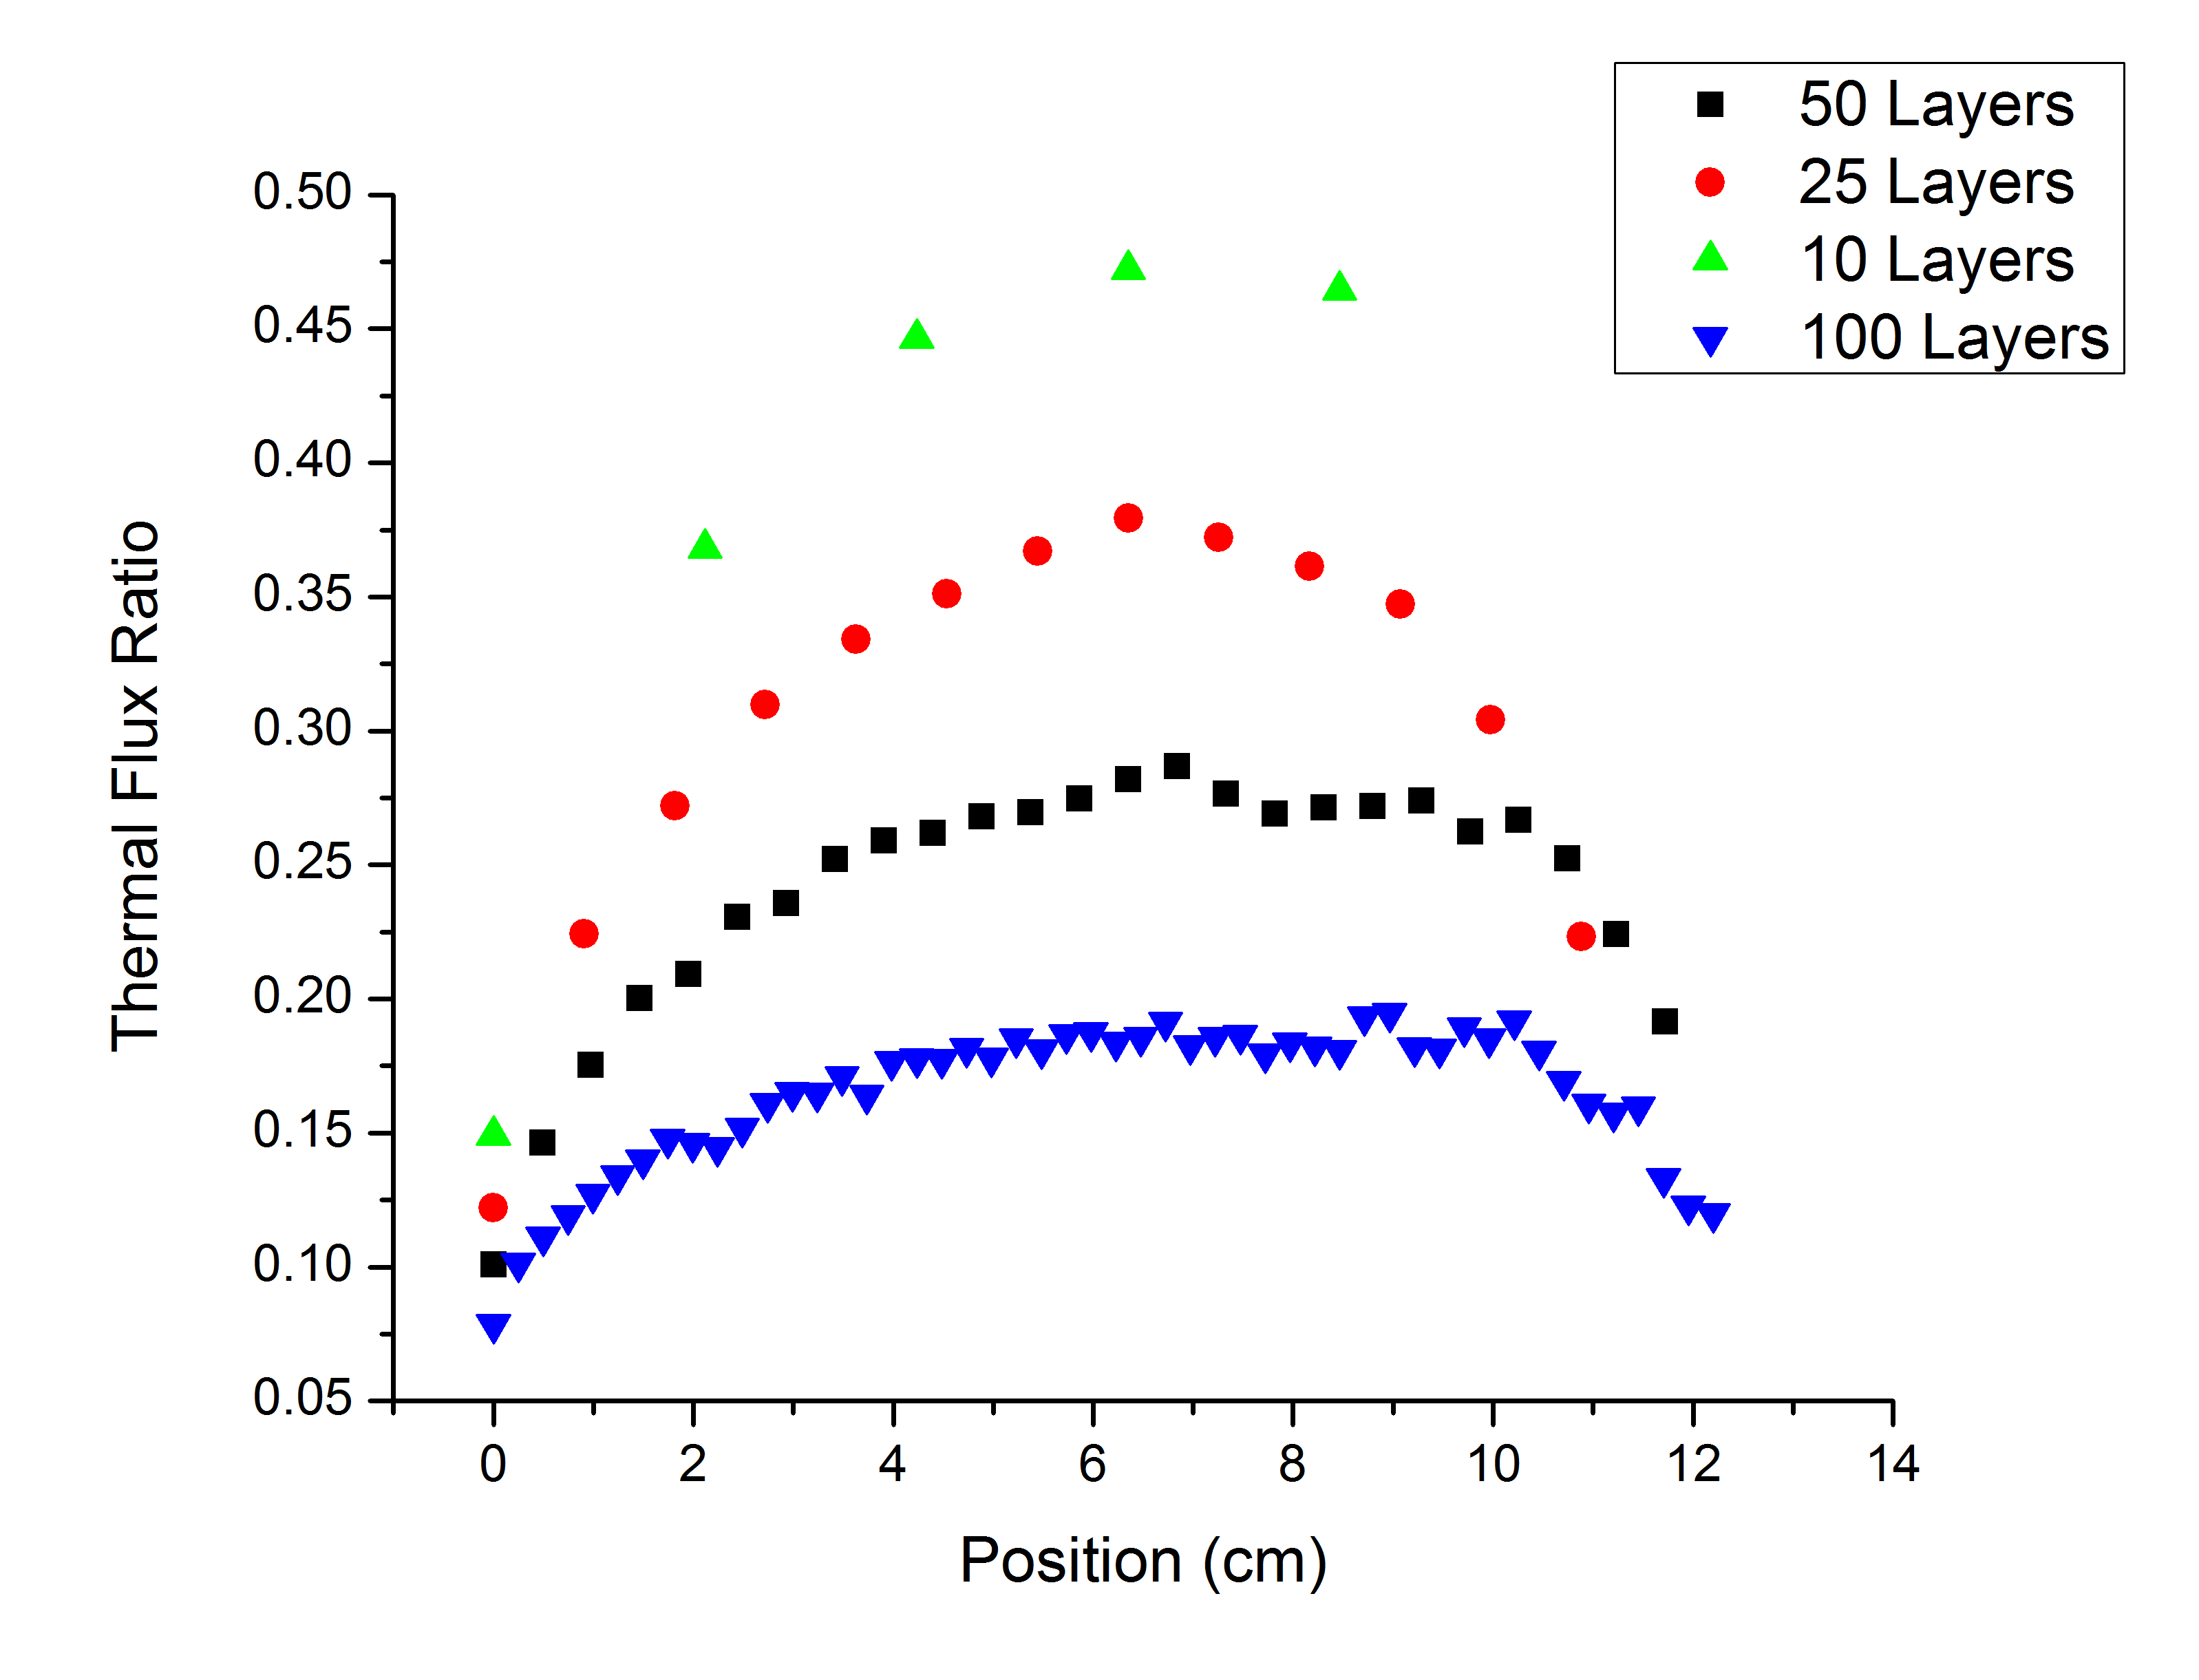
\includegraphics[width=\textwidth]{ThermalFluxRatioAltLayers}
	\caption{Fraction of the neutron flux that is thermalized through a alternating detector and moderator layered RPM.  The low thermal fluxes result in a poor utilization of the high thermal cross section of \iso[6]{Li}.}
	\label{fig:AltLayerThermalNeutronFraction}
\end{figure}
Effective utilization of the neutron flux is necessary for minimizing the amount of neutron absorber (\iso[6]{Li}) that is used in the detector.


\subsection{Optimal Layered Detector Geometries}
\label{sec:OptimalLayeredDetectorGeos}
The optimal genomes are listed for 10 15, 20 length, and 30 length genomes for a minimum interaction rate of 2.5 interactions per second in \autoref{tab:GAOptRXNRate_25}, 5.0 interactions per neutron per second in \autoref{tab:GAOptRXNRate_5}, and for 7.5 interactions per second in \autoref{tab:GAOptRXNRate_75}.
It is observed that higher length genomes tended to shows a slight decrease in the total interaction rate.

\begin{table}
	\caption[Optimal geometry for 2.5 interactions per second]{Optimal genome geometries for a total minimium interaction rate of 2.5 interactions per second. The detector and simulation is configured per the PNNL criteria.}
	\label{tab:GAOptRXNRate_25}
	\begin{tabular}{m{7cm} m{5cm} m{2cm} }
	\toprule
	Genome & Interaction Rate & Mass \iso[6]{Li} \\
	\midrule
	0011010000 & 3.82 & \SI{12.6}{\gram} \\
	00100101000000000000 & 3.79 &  \SI{12.6}{\gram}  \\
	00010100001000000000000000 & 3.75 &  \SI{12.6}{\gram}  \\
	\bottomrule
	\end{tabular}
\end{table}
\begin{table}
	\caption[Optimal geometry for 5 interactions per second]{Optimal genome geometries for a total minimum interaction rate of 5 interactions per second. The detector and simulation is configured per the PNNL criteria.}
	\label{tab:GAOptRXNRate_5}
	\begin{tabular}{m{7cm} m{5cm} m{2cm} }
	\toprule
	Genome & Interaction Rate  & Mass \iso[6]{Li} \\
	\midrule
	011101001000000 & 5.31 & \SI{21.0}{\gram} \\
	01011010010000000000 & 5.21& \SI{21.0}{\gram} \\
	011001001000010000000000000000 & 5.06 & \SI{21.0}{\gram} \\
	\bottomrule
	\end{tabular}
\end{table}
\begin{table}
	\caption[Optimal geometry for 7.5 interactions per second]{Optimal genome geometries for a total minimium interaction rate of 7.5 interactions per second. The detector and simulation is configured per the PNNL criteria.}
	\label{tab:GAOptRXNRate_75}
	\begin{tabular}{m{7cm} m{5cm} m{2cm} }
	\toprule
	Genome & Interaction Rate & Mass \iso[6]{Li} \\
	\midrule
	01111101110100001000 & 7.56 & \SI{41.2}{\gram} \\
	01111101010010101000 & 7.53 & \SI{41.2}{\gram} \\
	\bottomrule
	\end{tabular}
\end{table}

\begin{figure}
  \centering
  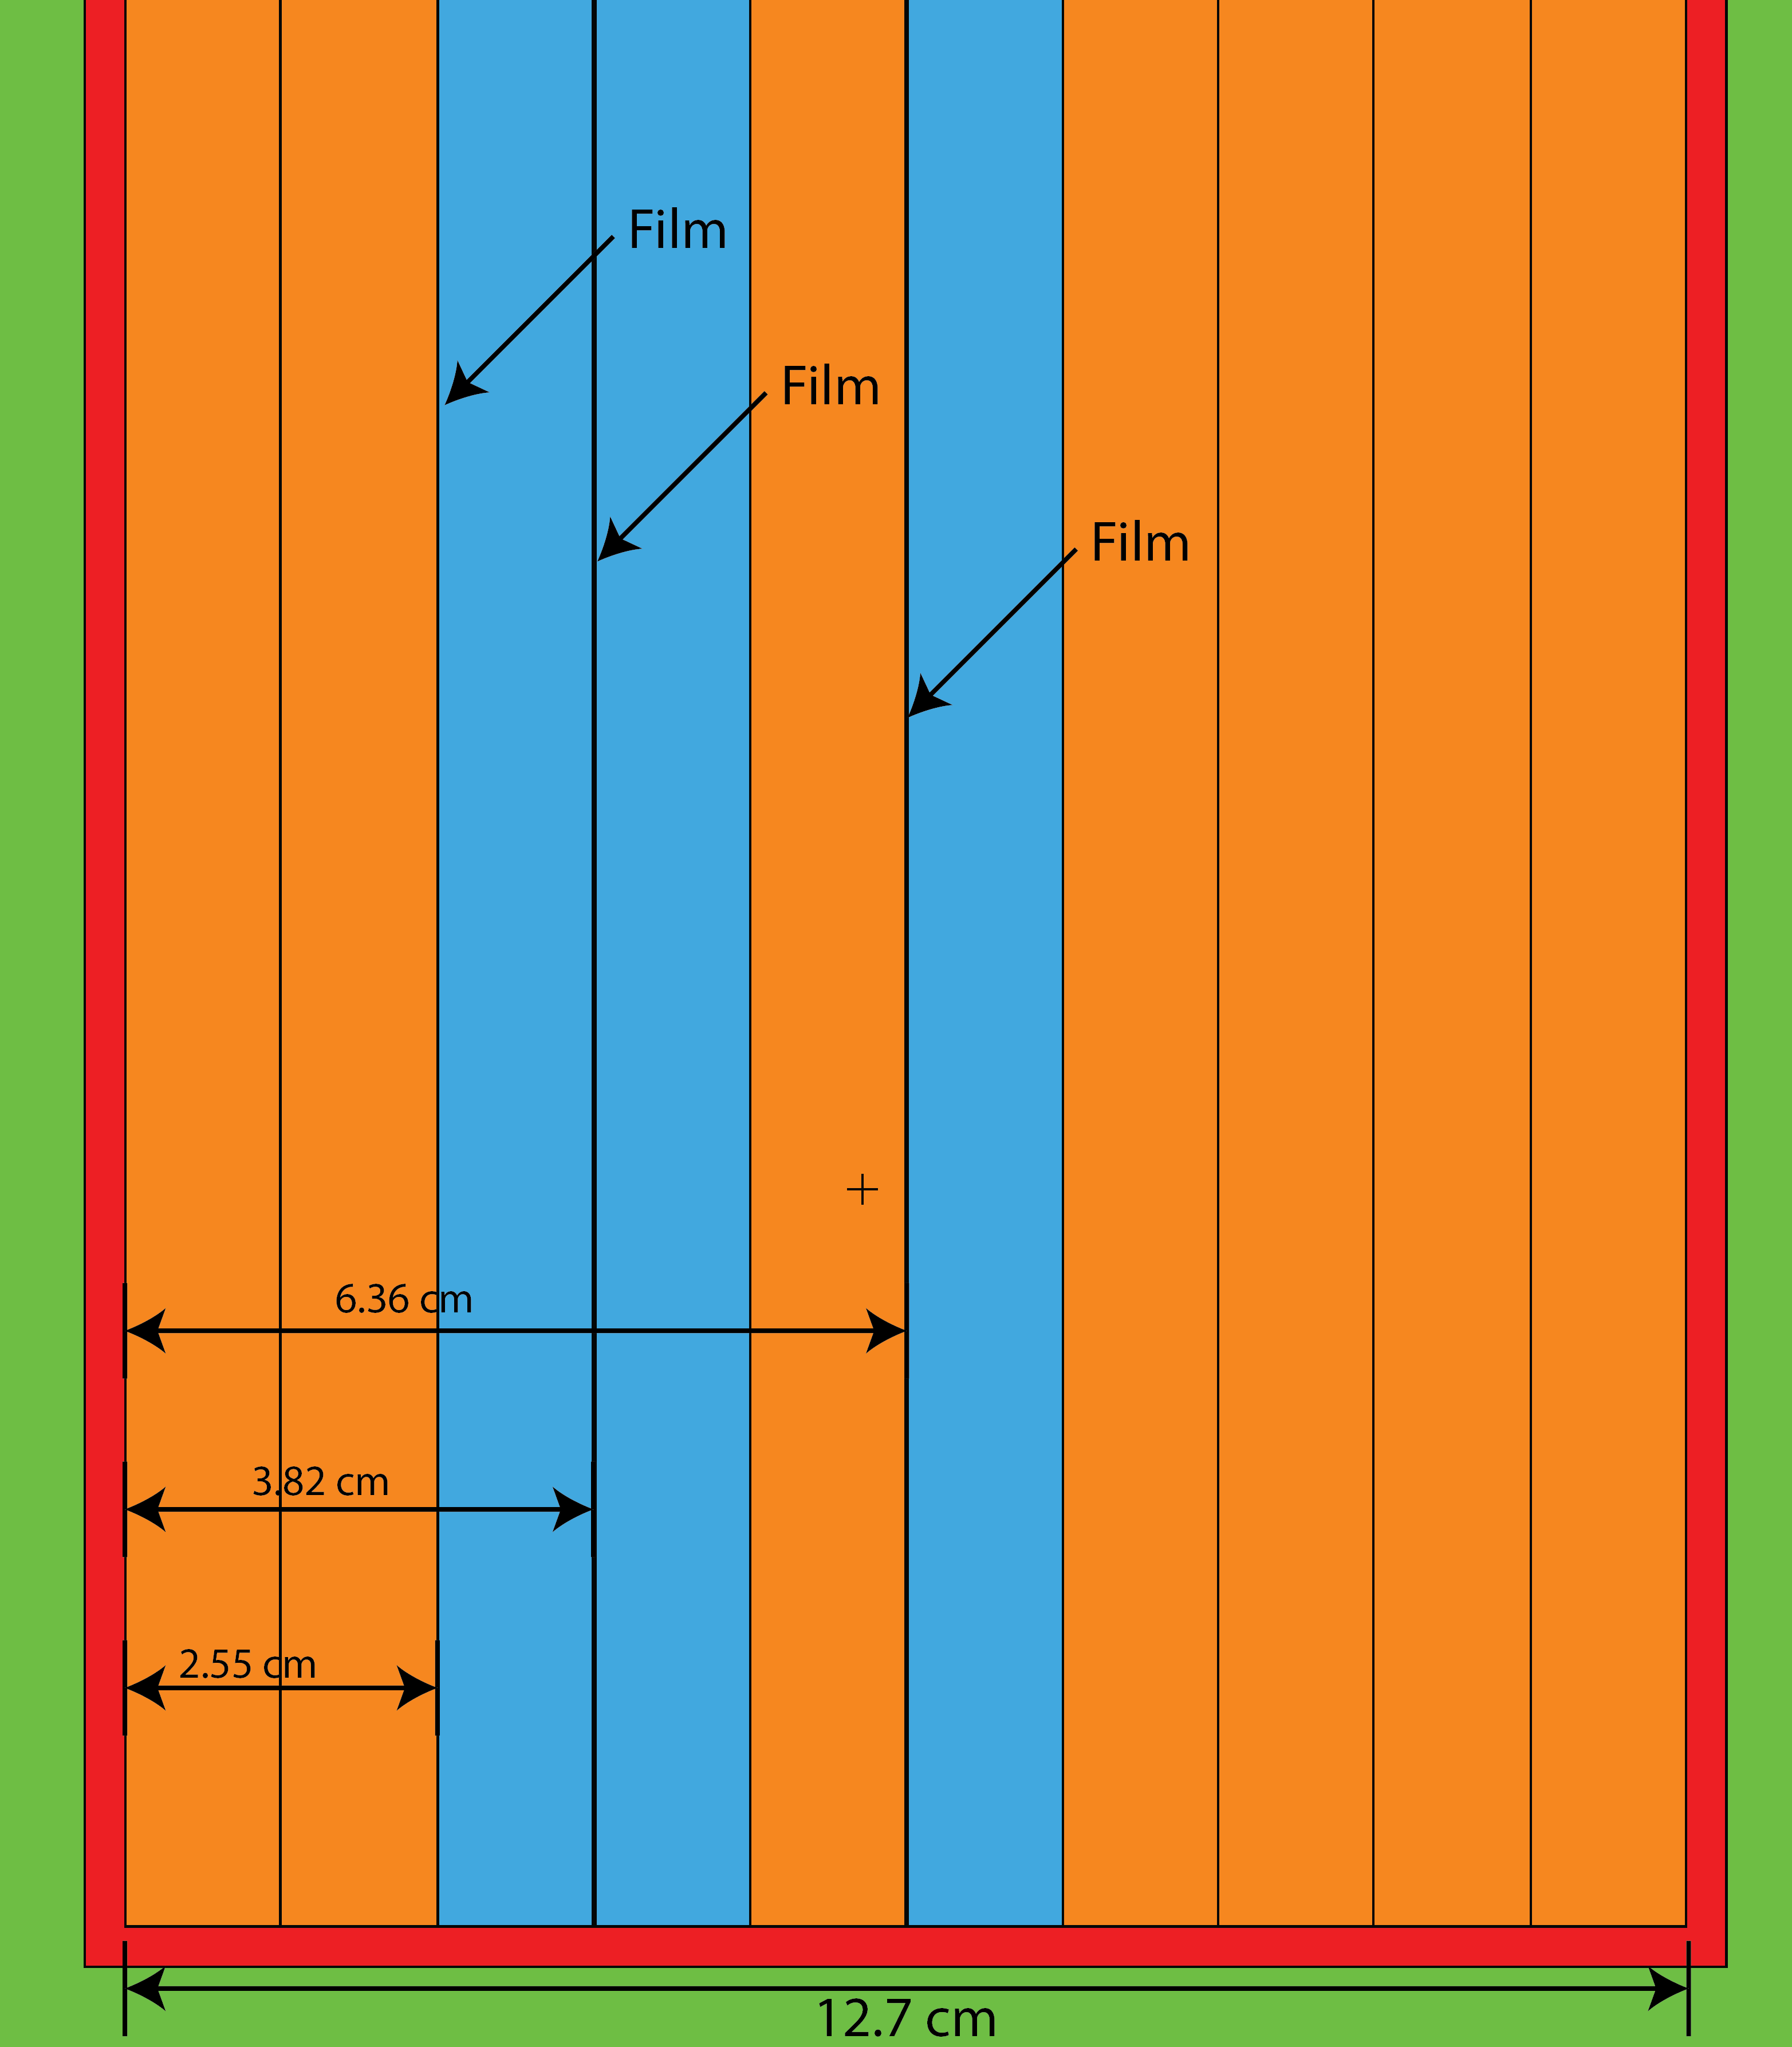
\includegraphics[width=\textwidth]{RPM8OptLayered_25cps}
  \caption[Position of Films in Optimized Layered RPM8 (2.5 interactions per nanogram Cf-252)]{Position of 10\% \iso[6]{Li} loaded polystyrene films in  an RPM8. The minimum count rate achieved in this configuration is 2.5 interactions per second per nanogram \iso[252]{Cf}.}
  \label{fig:RPMLayeredRendering25}
\end{figure}
\begin{figure}
  \centering
  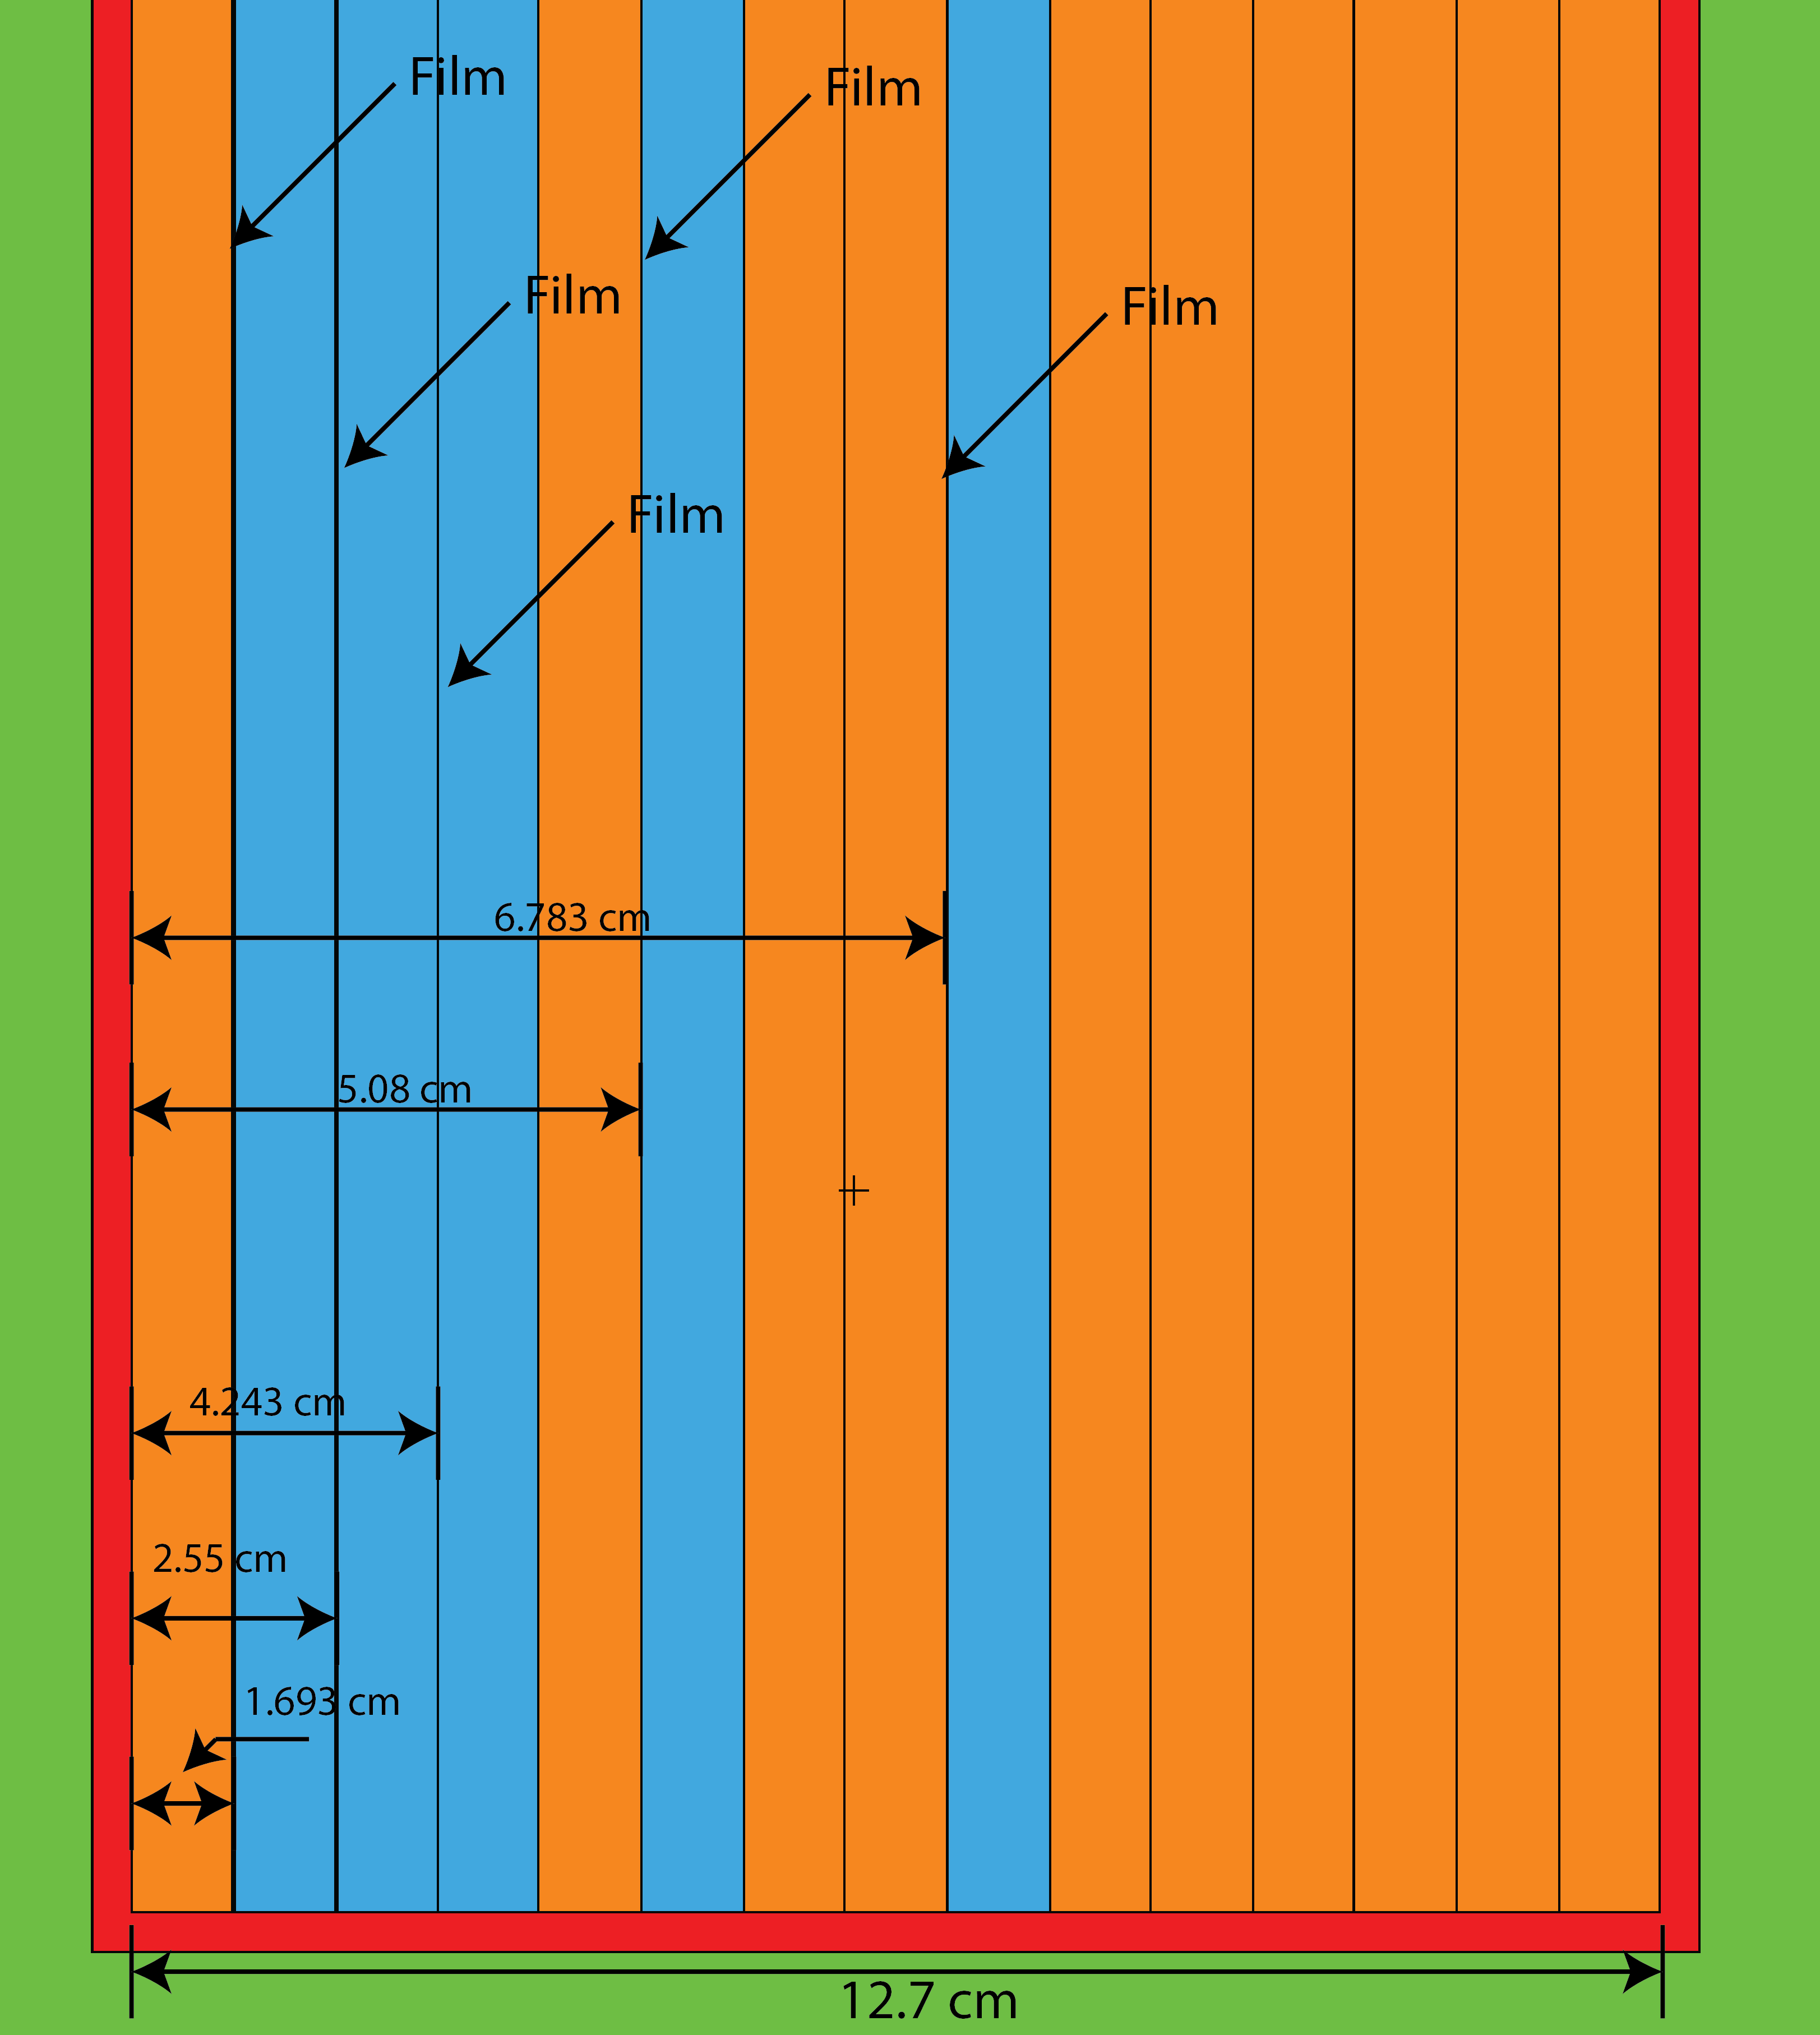
\includegraphics[width=\textwidth]{RPM8OptLayered_5cps}
  \caption[Position of Films in Optimized Layered RPM8 (5.0 interactions per nanogram Cf-252)]{Position of 10\% \iso[6]{Li} loaded polystyrene films in  an RPM8. The minimum count rate achieved in this configuration is 5.0 interactions per second per nanogram \iso[252]{Cf}.}
  \label{fig:RPMLayeredRendering5}
\end{figure}
\begin{figure}
  \centering
  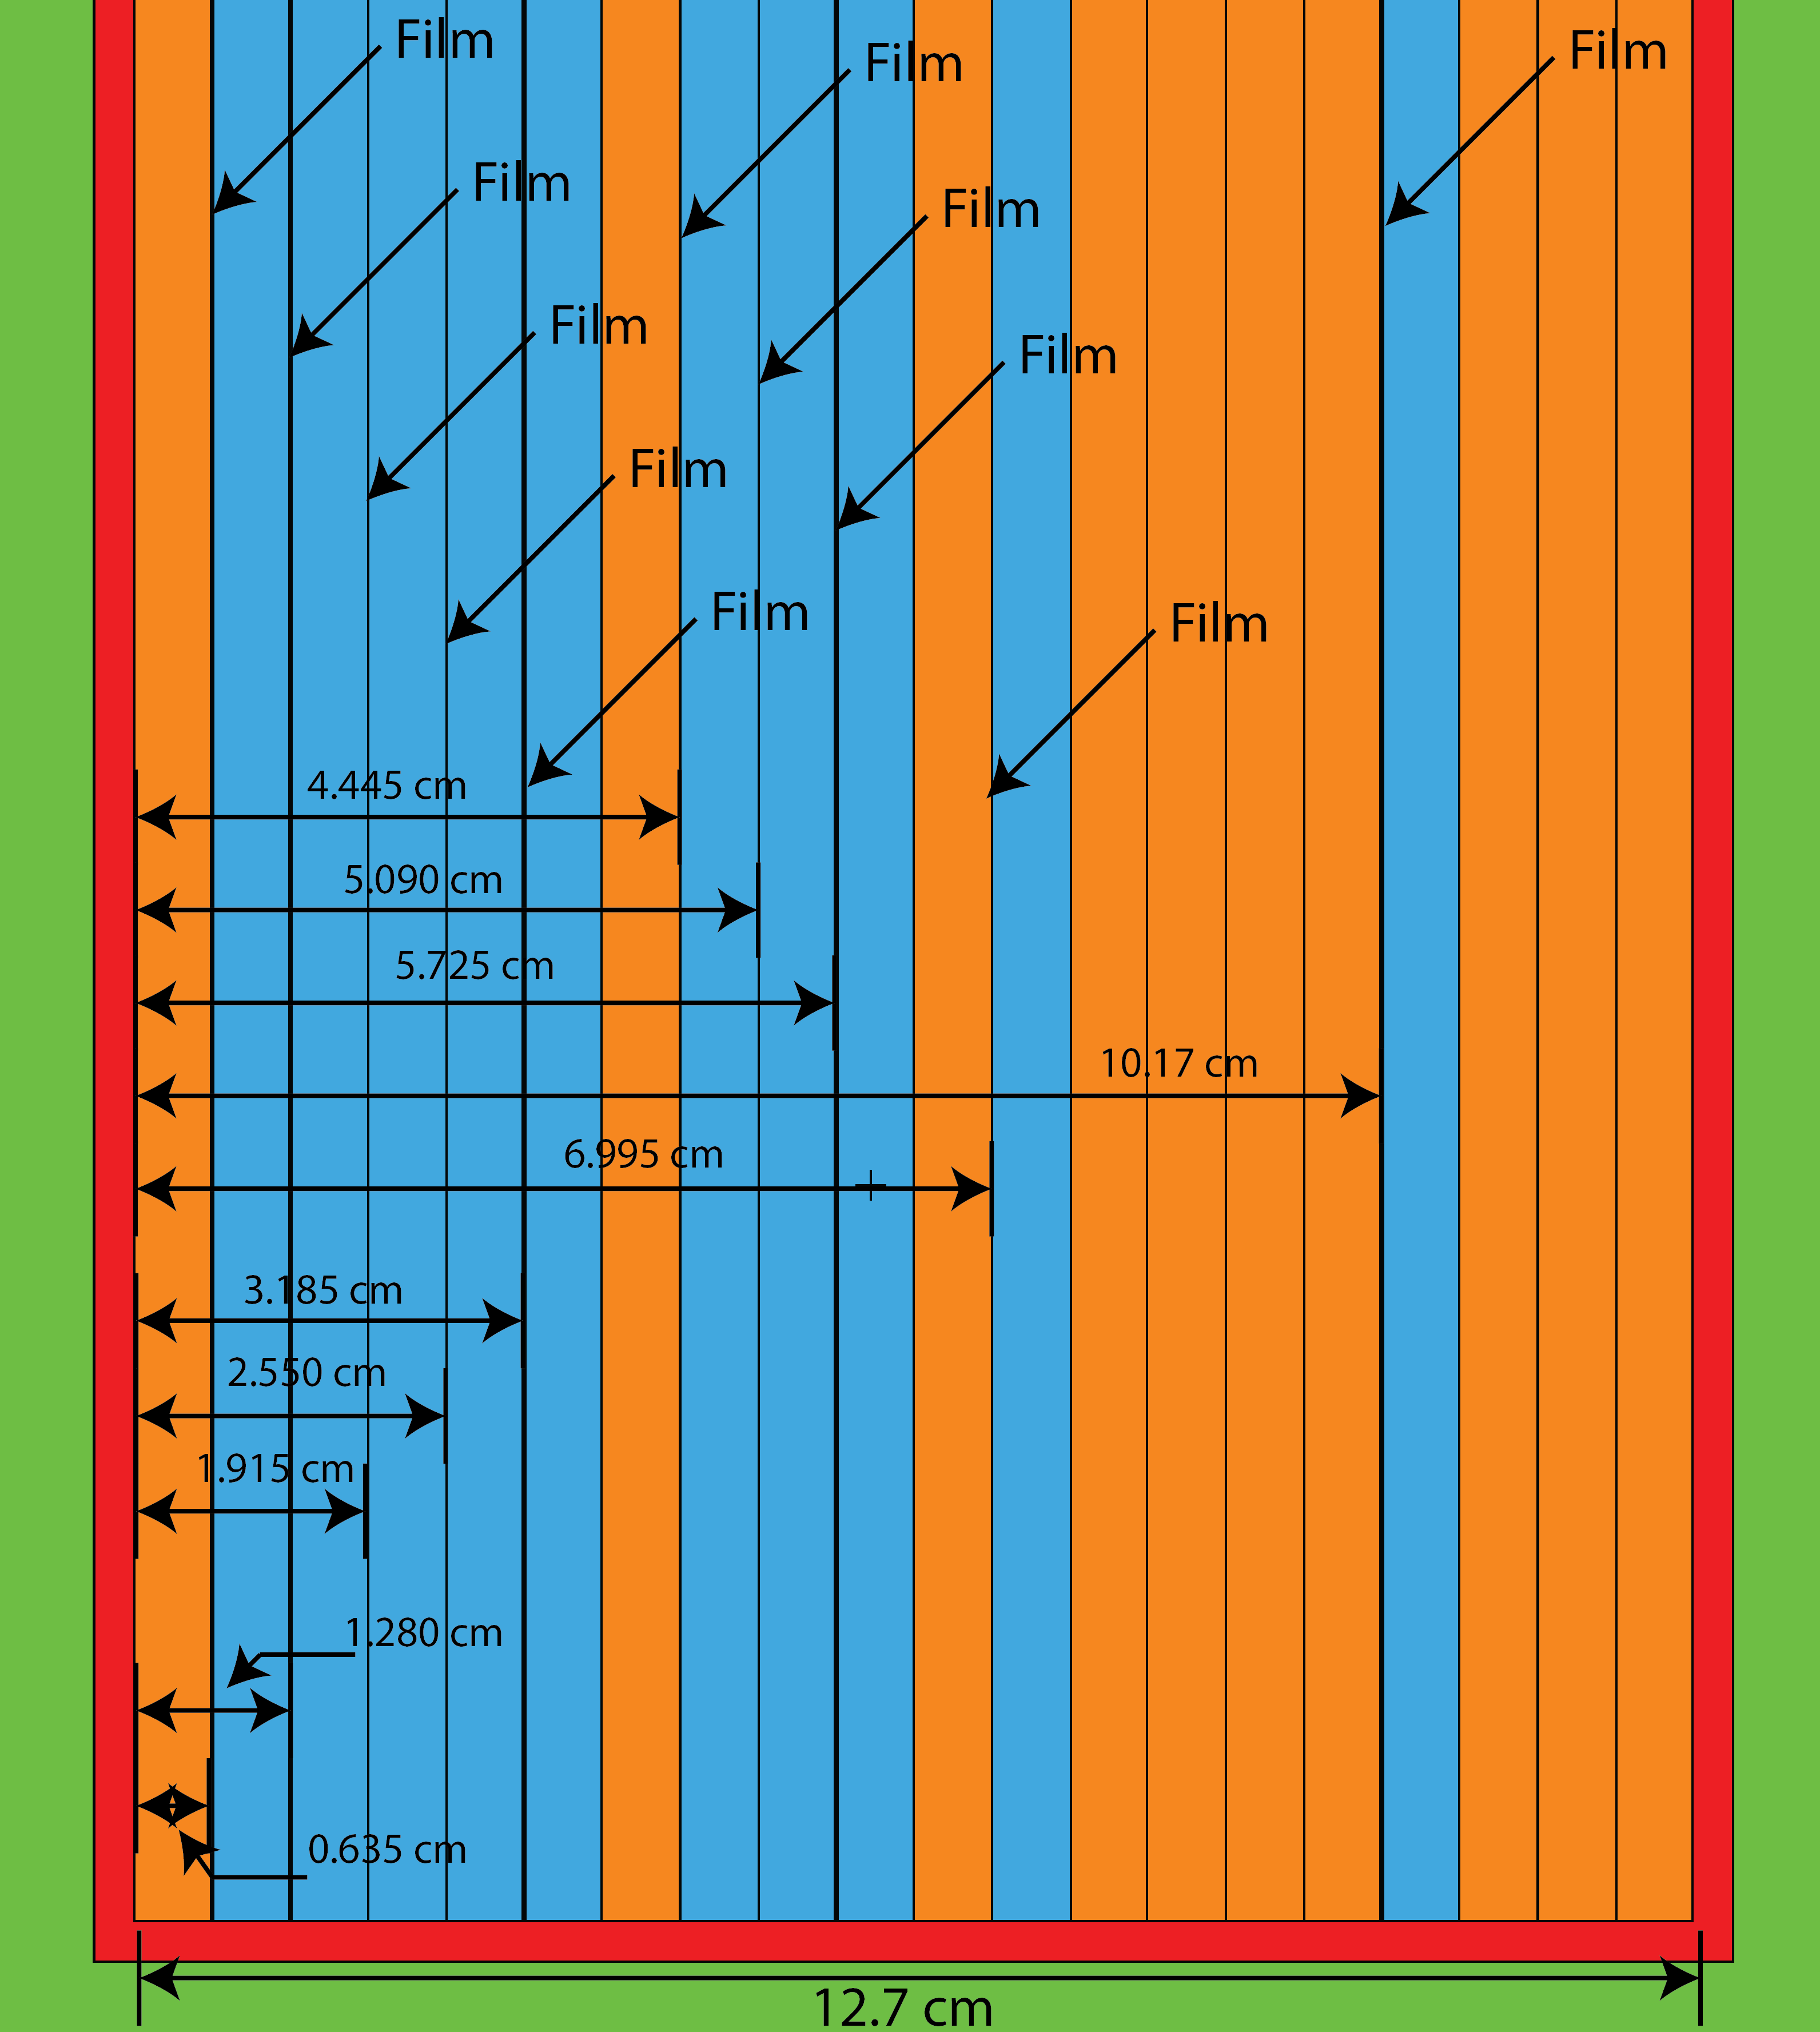
\includegraphics[width=\textwidth]{RPM8OptLayered_75cps}
  \caption[Position of Films in Optimized Layered RPM8 (7.5 interactions per nanogram Cf-252)]{Position of 10\% \iso[6]{Li} loaded polystyrene films in  an RPM8. The minimum count rate achieved in this configuration is 7.5 interactions per second per nanogram \iso[252]{Cf}.}
  \label{fig:RPMLayeredRendering75}
\end{figure}

The neutron flux as it crosses the detector is of interest to examine the utilization of the neutrons.
\autoref{fig:20Length25MinFluxProfile} shows the flux profiles for an optimal geometry for a 20 length genome with a minimum of 2.5 interactions per second and \autoref{fig:20Length5MinFluxProfile} shows the flux profiles for a minimum of 5 interactions per second.
It is observed that the fast flux quickly decreases as the there is a build up of the thermal flux.
Once the thermal flux has reached about \SI{4E-3}{neutrons \per \cm\squared \per\second} it is advantageous to place layers of \iso[6]{Li} to reduce the thermal flux.
A build up of the thermal flux is observed after the last detector layer, and the thermal flux declines as neutrons leave the detector.
\begin{figure}
	\centering
	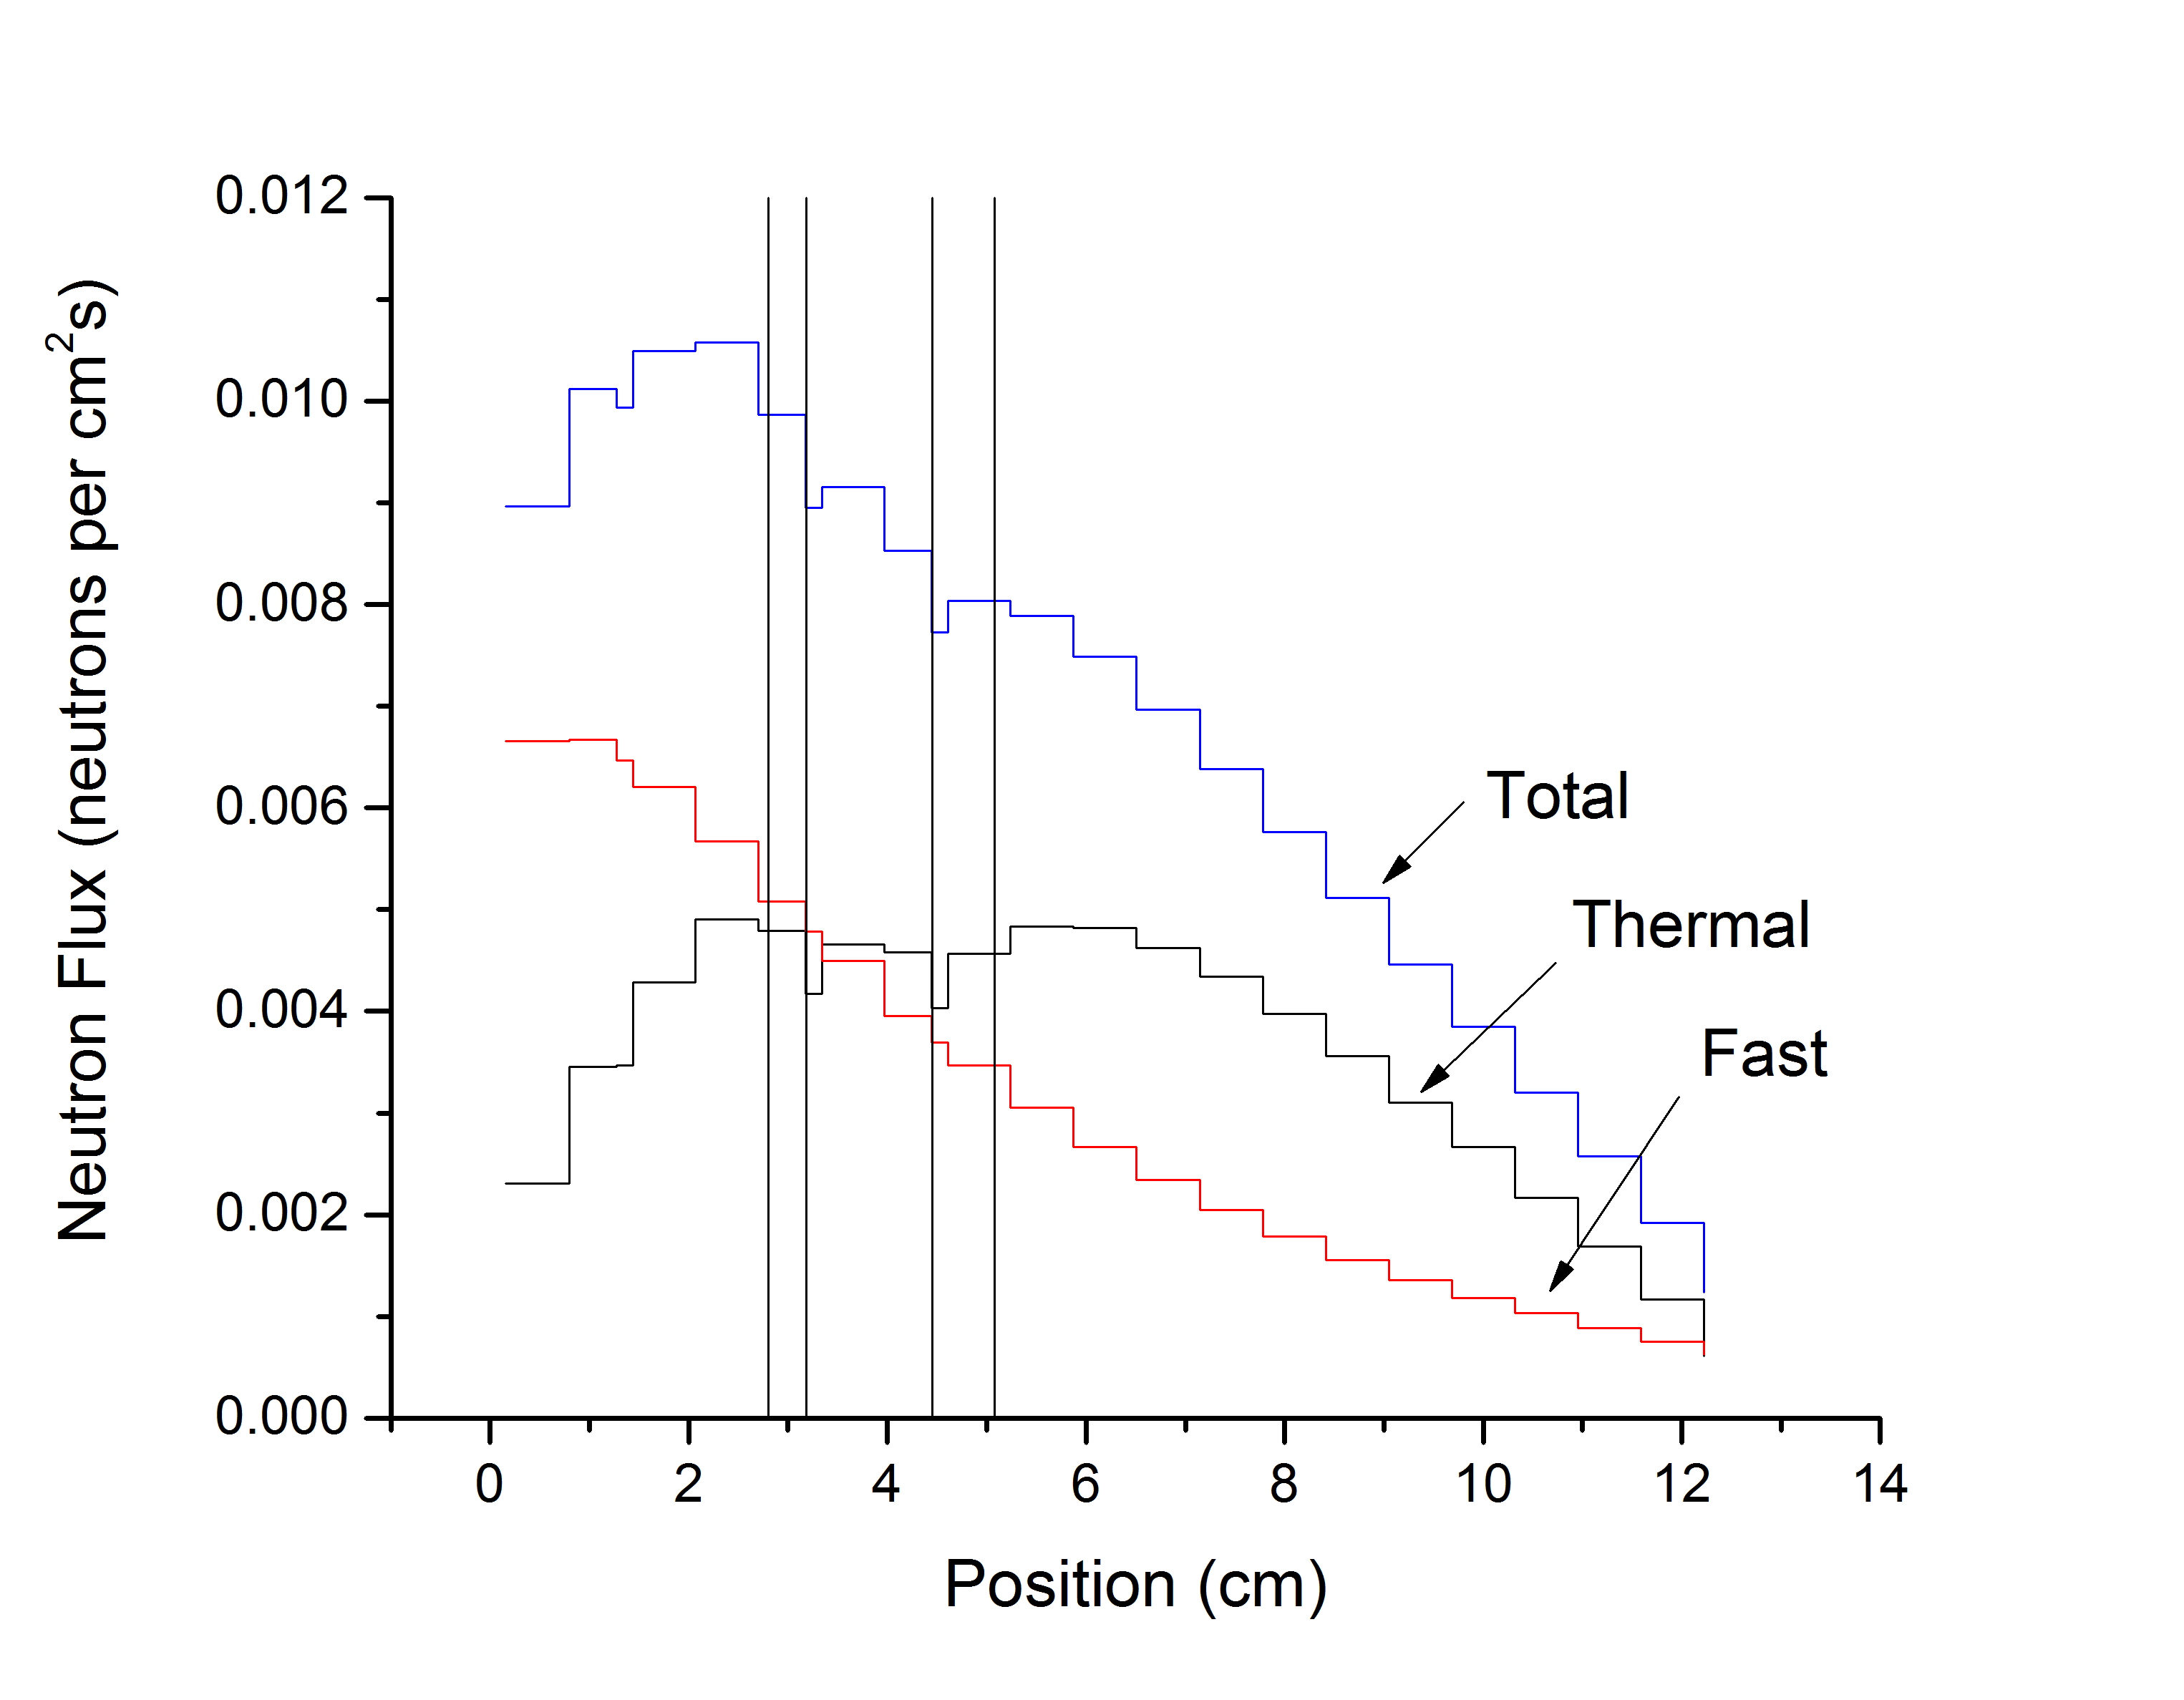
\includegraphics[width=\textwidth]{20Length25cpsMinFluxProfiles}
	\caption[Neutron Flux Profile for an Optimal 20 Length Genome, minimum 2.5 interactions per second]{Neutron flux profile for a 20 length genome with an interaction rate of 3.82 interactions per neutron. The vertical lines represent detector film layers.}
	\label{fig:20Length25MinFluxProfile}
\end{figure}
\begin{figure}
	\centering
	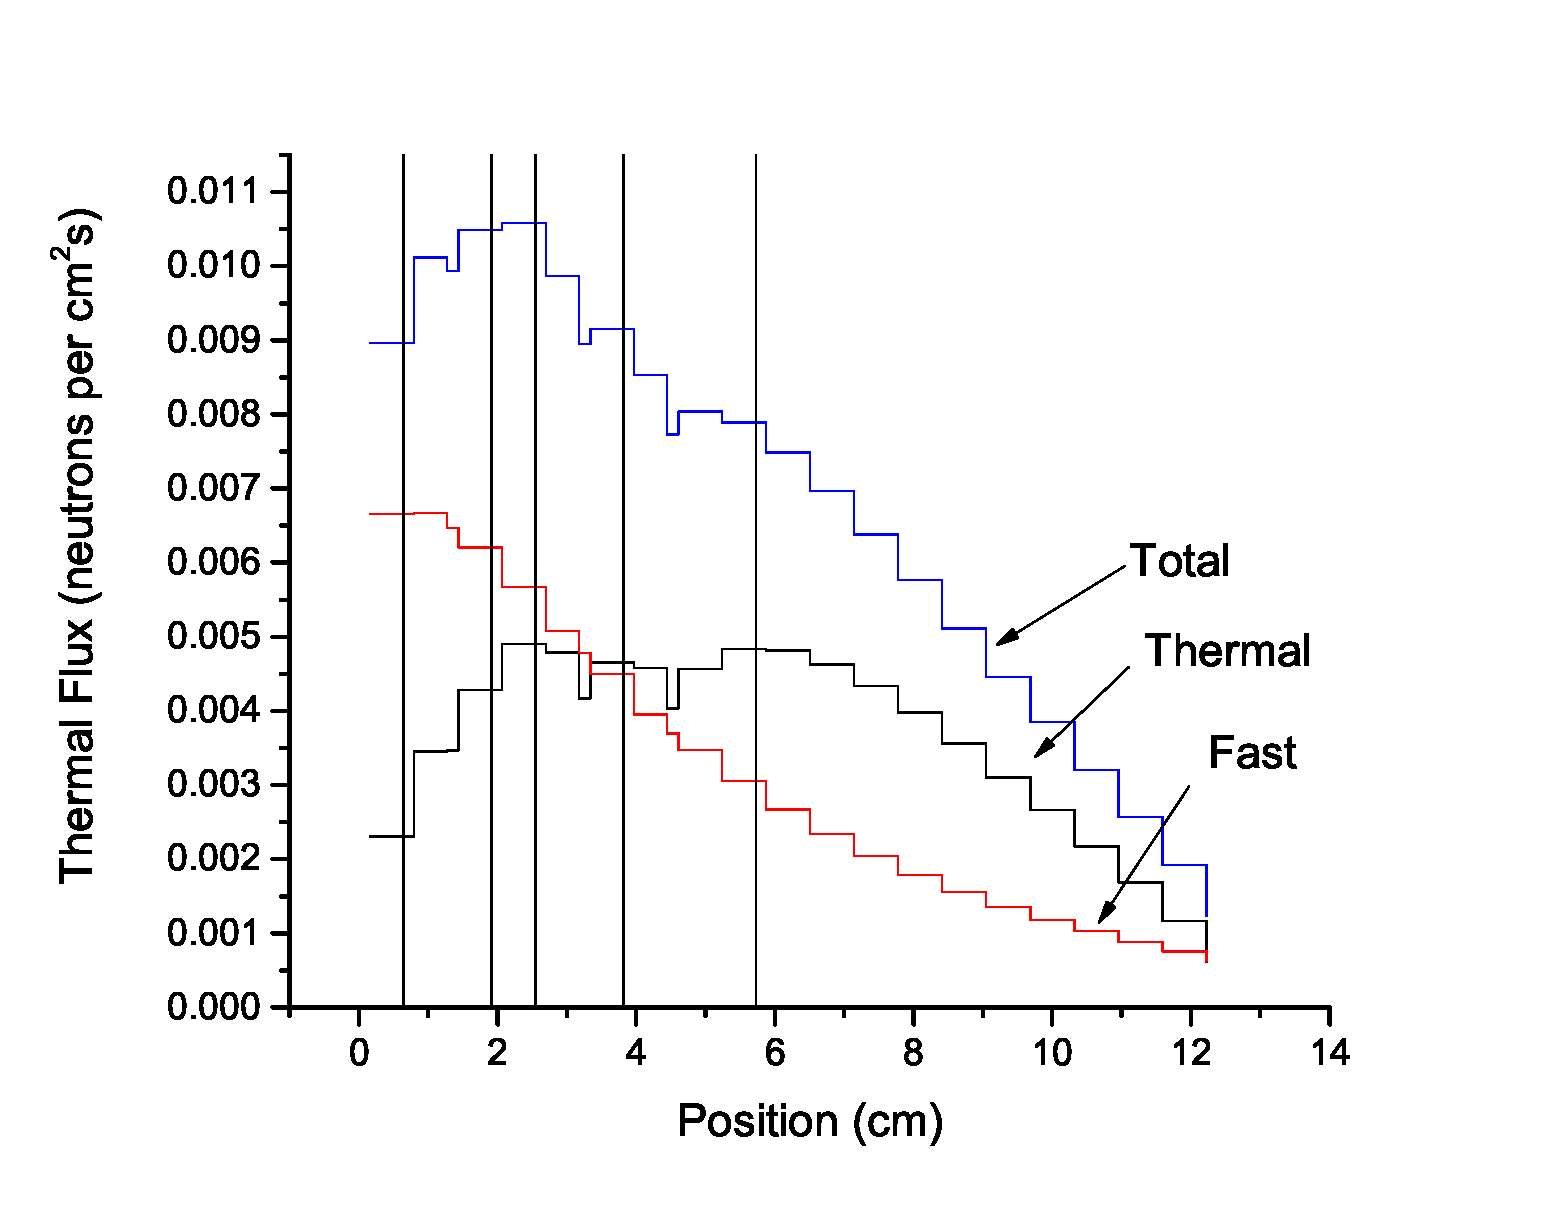
\includegraphics[width=\textwidth]{20Length5cpsMinFluxProfiles}
	\caption[Neutron Flux Profile for an Optimal 20 Length Genome, minimum 5 interactions per second]{Neutron flux profile for a 20 length genome with an interaction rate of 5.31 interactions per neutron. The vertical lines represent detector film layers.}
	\label{fig:20Length5MinFluxProfile}
\end{figure}

\begin{table}
	\caption[Optimal Layered Film Geometry for 7.5 interaction per second per nanogram Cf-252]{Optimal layered film geometry for an interaction rate of 7.5 interactions per second per nano-gram \iso[252]{Cf} in a 10\% \iso[6]{Li} loaded PS film. The positions shown in the table are the right boundary, where the detector starts at \SI{0.0}{\cm}. The genome representing this geometry is \texttt{01111101110100001000}.}
	\label{tab:OptGeoDetailed75}
	\begin{tabular}{m{3cm} m{4cm}}
	\toprule
	Position (\si{\cm}) & Material \\
	\midrule
0.635&Moderator\\
0.645&Detector\\
1.270&LightGuide\\
1.280&Detector\\
1.905&LightGuide\\
1.915&Detector\\
2.540&LightGuide\\
2.550&Detector\\
3.175&LightGuide\\
3.185&Detector\\
3.810&LightGuide\\
4.445&Moderator\\
4.455&Detector\\
5.080&LightGuide\\
5.090&Detector\\
5.715&LightGuide\\
5.725&Detector\\
6.350&LightGuide\\
6.985&Moderator\\
6.995&Detector\\
7.620&LightGuide\\
8.255&Moderator\\
10.170&Detector\\
10.795&LightGuide\\
11.430&Moderator\\
	\bottomrule
	\end{tabular}
\end{table}
\begin{table}
	\caption[Optimal Layered Film Geometry for 5.0 interaction per second per nanogram Cf-252]{Optimal layered film geometry for an interaction rate of 5.0 interactions per second per nano-gram \iso[252]{Cf}  in a 10\% \iso[6]{Li} loaded PS film. The positions shown in the table are the right boundary, where the detector starts at \SI{0.0}{\cm}. The genome representing this geometry is \texttt{011101001000000}.}
	\label{tab:OptGeoDetailed5}
	\begin{tabular}{m{3cm} m{4cm}}
	\toprule
	Position (\si{\cm}) & Material \\
	\midrule
0.847&Moderator\\
0.857&Detector\\
1.693&LightGuide\\
1.703&Detector\\
2.540&LightGuide\\
2.550&Detector\\
3.387&LightGuide\\
4.233&Moderator\\
4.243&Detector\\
5.080&LightGuide\\
5.927&Moderator\\
6.783&Detector\\
7.620&LightGuide\\
8.467&Moderator\\
	\bottomrule
	\end{tabular}
\end{table}
\begin{table}
	\caption[Optimal Layered Film Geometry for 2.5 interaction per second per nanogram Cf-252]{Optimal layered film geometry for an interaction rate of 2.5 interactions per second per nano-gram \iso[252]{Cf} in a 10\% \iso[6]{Li} loaded PS film. The positions shown in the table are the right boundary, where the detector starts at \SI{0.0}{\cm}. The genome representing this geometry is \texttt{0011010000}.}
	\label{tab:OptGeoDetailed25}
	\begin{tabular}{m{3cm} m{4cm}}
	\toprule
	Position (\si{\cm}) & Material \\
	\midrule
1.270&Moderator\\
2.550&Detector\\
3.810&LightGuide\\
3.820&Detector\\
5.080&LightGuide\\
6.350&Moderator\\
6.360&Detector\\
7.620&LightGuide\\
8.890&Moderator\\
	\bottomrule
	\end{tabular}
\end{table}

\subsection{Wrapped Polymer Cylinders}
\label{sec:WrappedCylinders}

In addition to planar detector sheets a possible replacement geometry could be to wrap the detector sheets around a wavelength shifting light core in concentric cylinders and replace the helium tube directly.
MCNPX simulations were completed of geometries containing two, three, and four cylinders of wrapped detector material.
It is envisioned that the detector material could be deposited on a flexible sheet and wrapped to create a cylinder, however, for simplicity a concentric cylinder design is simulated.
The outer diameter of the cylinders were set to be two inches (\SI{2.5}{\cm}) to be a direct replacement of the existing helium three tubes.
The exact placement of the helium tubes in an RPM is not known, so the tubes were placed one-third of the way back in the detector material, and spaced equidistance apart.
The spacing of the tubes inside the radiation portal monitor is described in \autoref{tab:WrappedCylinderPositions}, and shown in \autoref{fig:WrappedCylinderGeo} and \autoref{fig:WrappedCylinderPos}.
\begin{figure}
  \centering
  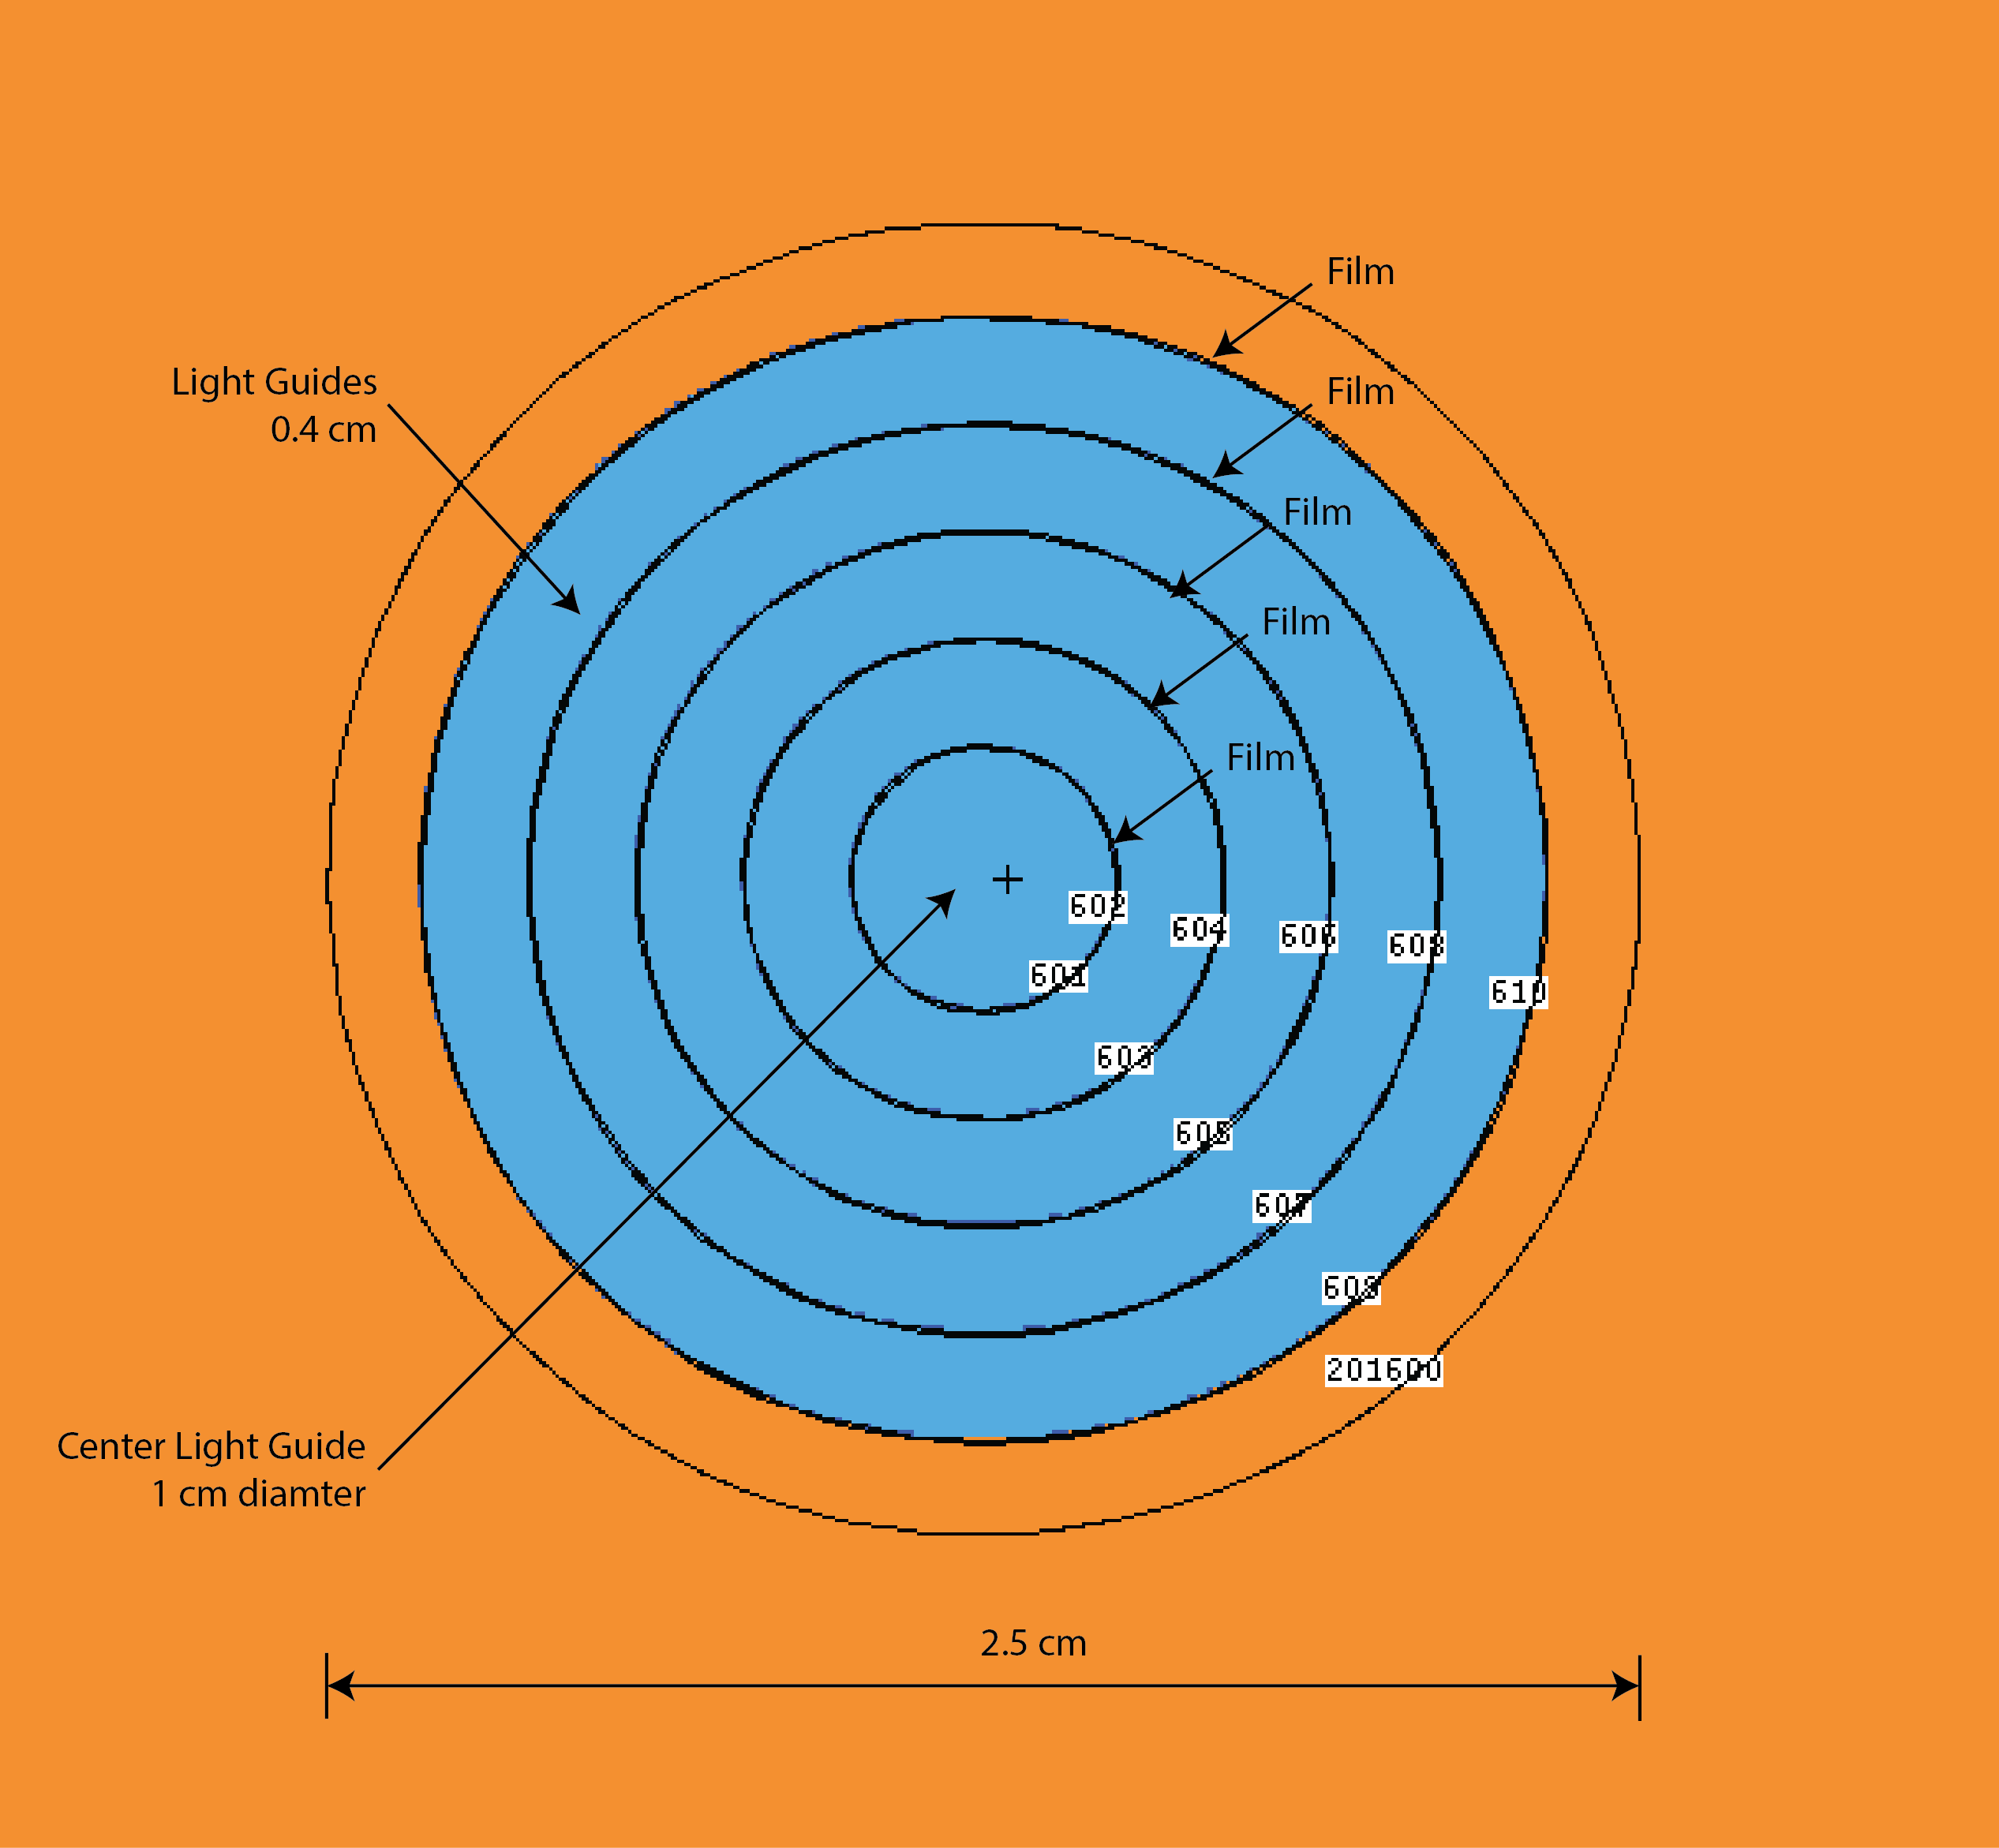
\includegraphics[width=\textwidth,height=\textheight,keepaspectratio]{WrappedGeoCylinder_Cylinder}
  \caption[Rendering of Wrapped Cylinder Geometry]{MCNPX Rendering of a wrapped cylinder.  There is a \SI{1}{\cm} diameter inner light guide surrounded by films separated by \SI{0.4}{\cm} thick light guides.}
  \label{fig:WrappedCylinderGeo}
\end{figure}
\begin{figure}
  \centering
  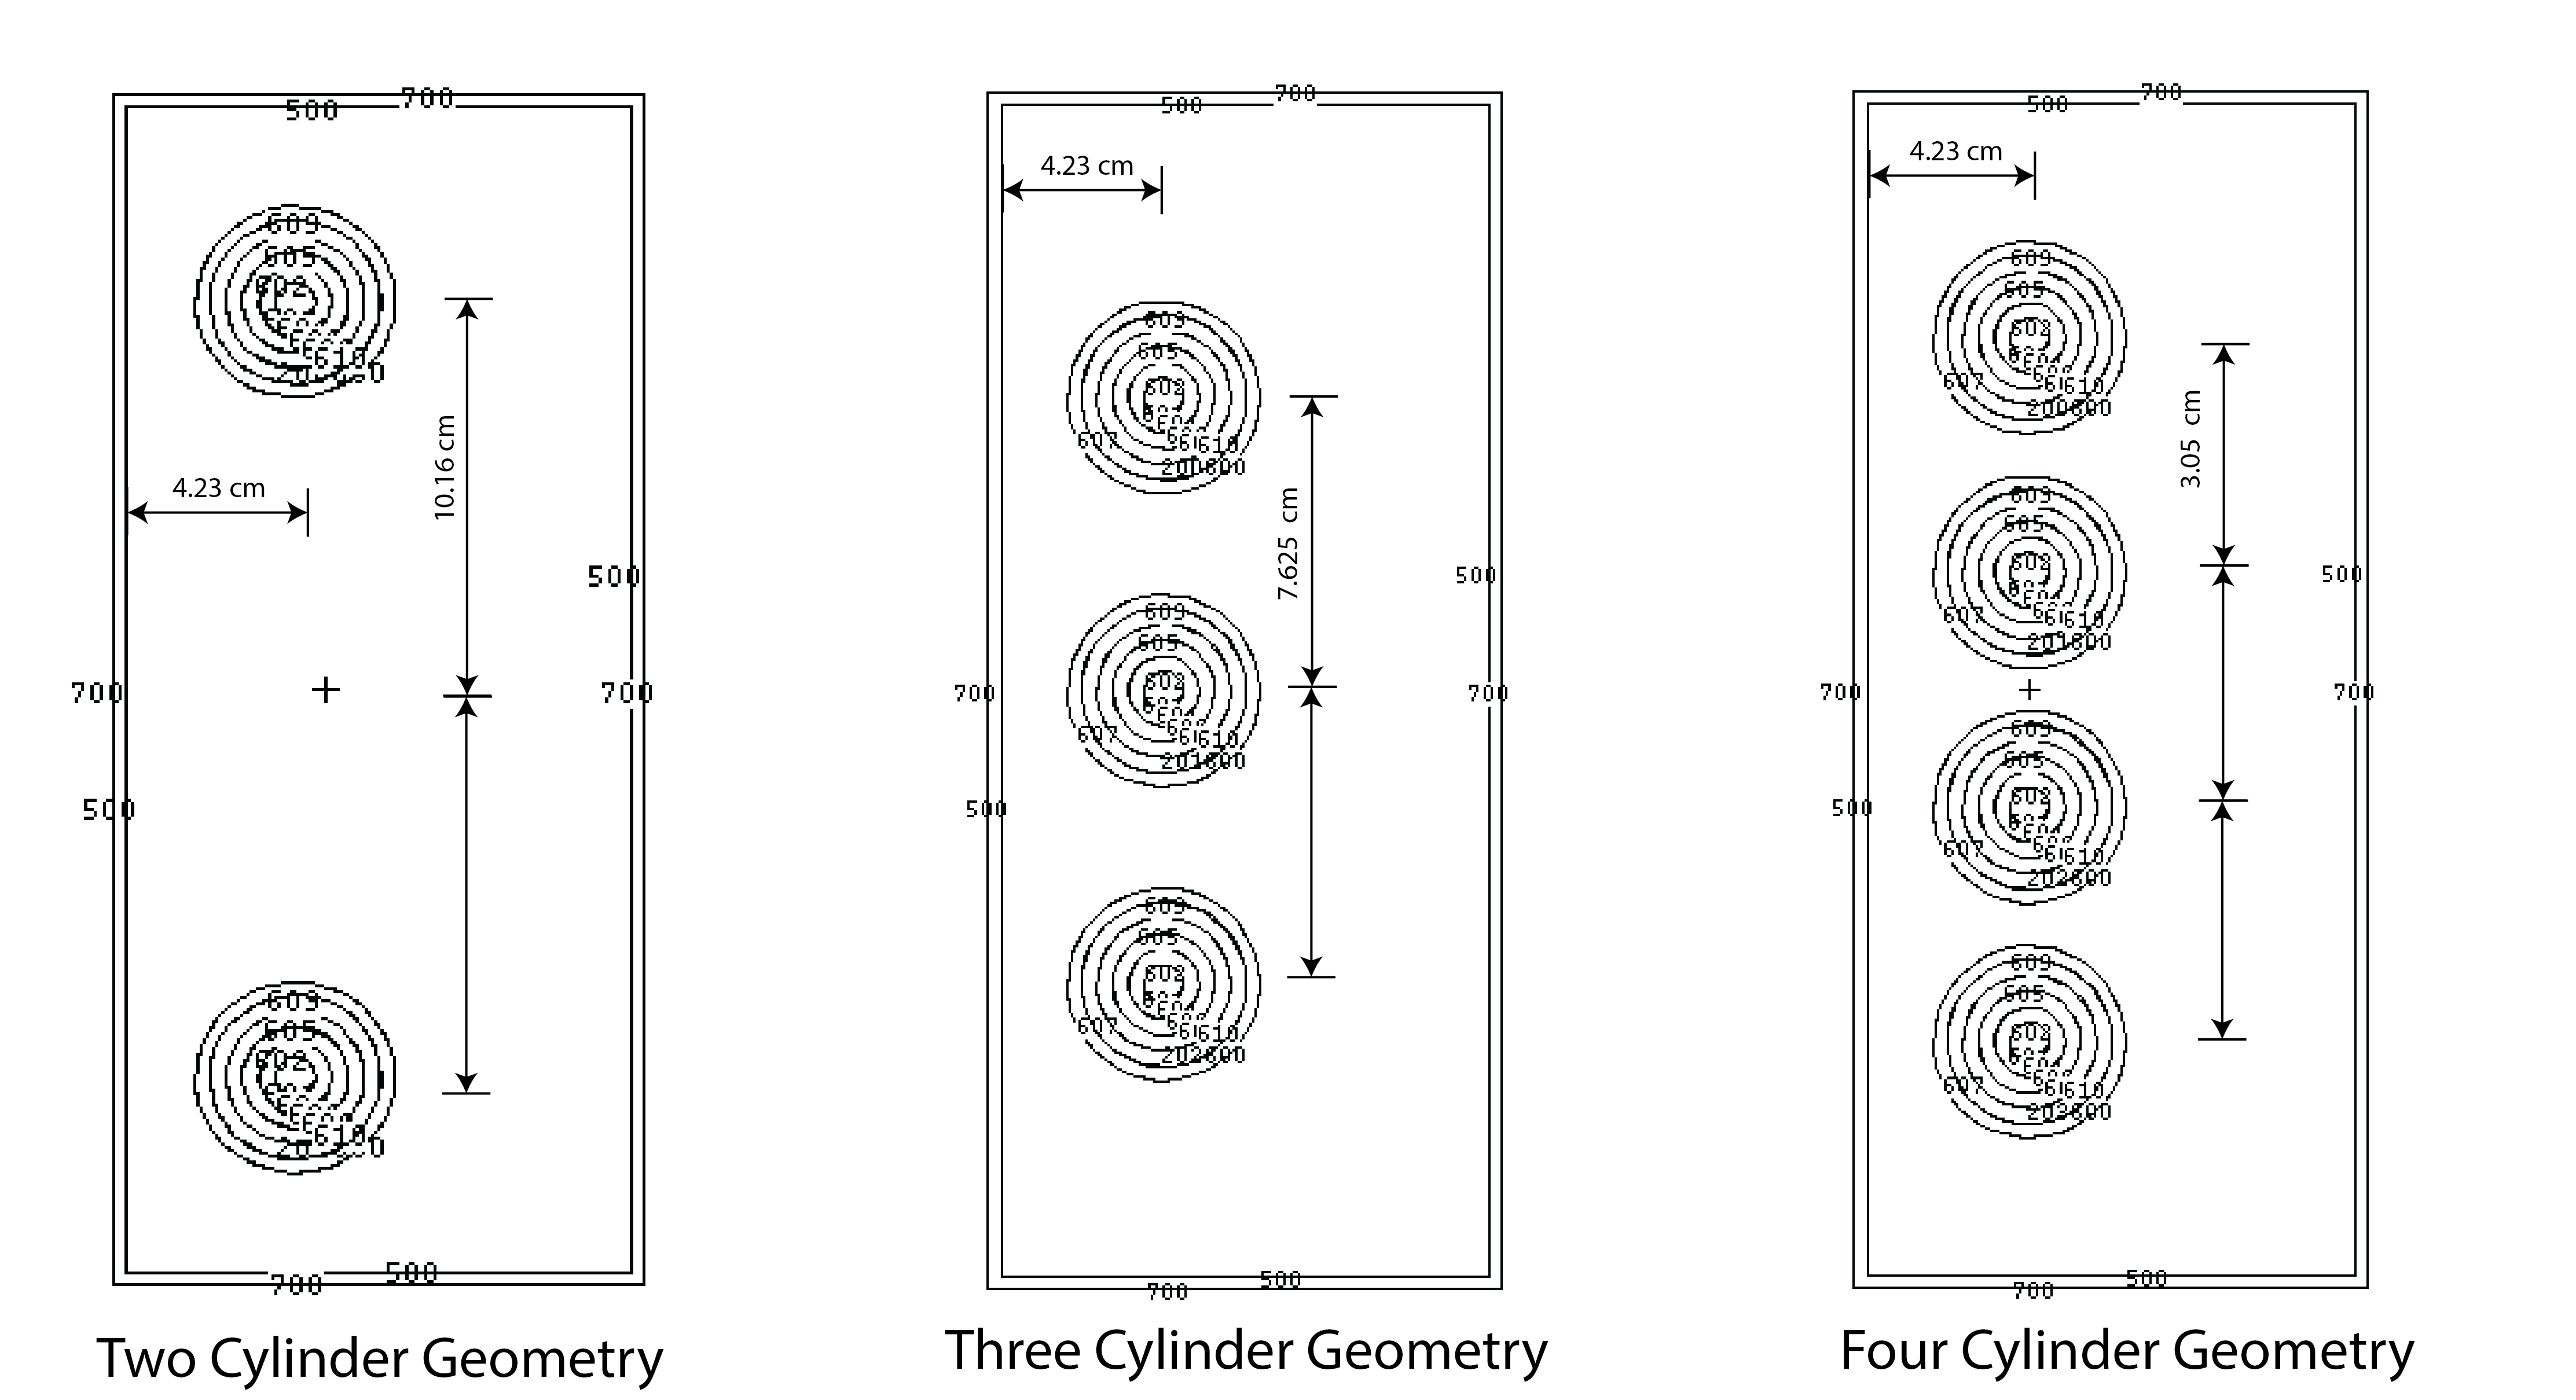
\includegraphics[width=\textwidth]{WrappedGeoCylinder_Positions}
  \caption[Positions of Wrapped Cylinders in RPM Cabinet]{MCNPX Rendering of wrapped cylinders placed in an RPM8 Cabinet.}
  \label{fig:WrappedCylinderPos}
\end{figure}
The thickness of the RPM (\SI{12.7}{\cm}) corresponds to the x dimension, where the front of the detector is at x equals \SI{0.0}{\cm}.
The width of the RPM cabinet extends from \SI{-15.25}{\cm} to \SI{15.25}{\cm}, where a y coordinate of zero is on the midline of the detector width.
\begin{table}
  \caption[Wrapped Cylinder Positions]{Positions of the wrapped cylinders in the RPM. The thickness of the RPM corresponds to the x dimension, and the width of the RPM cabinet extends from \SI{-15.25}{\cm} to \SI{15.25}{\cm}}
  \label{tab:WrappedCylinderPositions}
  \begin{tabular}{m{2cm} | m{3cm} m{4cm} }
    \toprule
    Number Cylinders & x coordinate & y coordinate \\
    \midrule
    2 & \SI{4.23}{\cm} & $\pm$ \SI{10.16}{\cm} \\
    3 & \SI{4.23}{\cm} & \SI{0}{\cm}, $\pm$ \SI{7.625}{\cm} \\
    4 & \SI{4.23}{\cm} & $\pm$ \SI{3.05}{\cm}, $\pm$ \SI{9.15}{\cm} \\
    \bottomrule
  \end{tabular}
\end{table}
\begin{table}
  \caption[Two Wrapped Cylinders Interaction Rate]{MCNPX simulated interaction rate of two wrapped cylinders of polymer loaded \iso[6]{LiF} in the RPM8 footprint}
  \label{tab:TwoCylinderResults}
	\begin{tabular}{m{2cm} >{\centering\arraybackslash} m{2cm} >{\centering\arraybackslash} m{2cm} >{\centering\arraybackslash} m{4cm} >{\centering\arraybackslash} m{4cm} }
	\toprule
    Polymer& Fraction \iso[6]{LiF} & Mass \iso[6]{Li}& Interaction Rate  & Count Rate per Mass \\
           &                       &  \centering{\si{\gram}} & \si{\cps\per\ng} \iso[255]{Cf}  & \si{\cps\per\ng \iso[252]{Cf}\per\gram} \\
    \midrule
    PS     &  0.10  & 4.80 &    1.321  $\pm$   0.03 &   0.28\\ 
    PS     &  0.20  &  9.60 &   1.852  $\pm$   0.04 &   0.19\\
    PS     &  0.30  &  14.38 &  2.160 $\pm$   0.04 &   0.15\\
    PEN    &  0.10&  4.77 &   1.325  $\pm$   0.03 &   0.28\\
    PEN    &  0.20&  9.54 &   1.841  $\pm$   0.04 &   0.19\\
    PEN    &  0.30&  14.31 &  2.157 $\pm$   0.04 &   0.15\\ 
    \bottomrule
  \end{tabular}
\end{table}

\begin{table}
  \caption[Three Wrapped Cylinders Interaction Rate]{MCNPX simulated interaction rate of three wrapped cylinders of polymer loaded \iso[6]{LiF} in the RPM8 footprint}
  \label{tab:ThreeCylinderResults}
	\begin{tabular}{m{2cm} >{\centering\arraybackslash} m{2cm} >{\centering\arraybackslash} m{2cm} >{\centering\arraybackslash} m{4cm} >{\centering\arraybackslash} m{4cm} }
	\toprule
    Polymer& Fraction \iso[6]{LiF} & Mass \iso[6]{Li}& Interaction Rate  & Count Rate per Mass \\
           &                       &  \centering{\si{\gram}} & \si{\cps\per\ng} \iso[255]{Cf}  & \si{\cps\per\ng \iso[252]{Cf}\per\gram} \\
    \midrule
    PS     &  0.10  & 7.20&   1.482   $\pm$  0.02 &   0.21\\
    PS     &  0.20  & 14.39&   2.240 $\pm$  0.03 &   0.16\\
    PS     &  0.30  & 21.58&   2.706 $\pm$  0.04 &   0.13\\
   PEN    &  0.10  & 7.15&   1.368  $\pm$  0.02 &   0.19\\
   PEN    &  0.20  &14.31 &  2.119 $\pm$  0.03 &   0.15\\
   PEN    &  0.30  &21.46 &  2.608 $\pm$  0.04 &  0.12 \\
    \bottomrule
  \end{tabular}
\end{table}

\begin{table}
  \caption[Four Wrapped Cylinders Interaction Rate]{MCNPX simulated interaction rate of four wrapped cylinders of polymer loaded \iso[6]{LiF} in the RPM8 footprint}
  \label{tab:FourCylinderResults}
	\begin{tabular}{m{2cm} >{\centering\arraybackslash} m{2cm} >{\centering\arraybackslash} m{2cm} >{\centering\arraybackslash} m{4cm} >{\centering\arraybackslash} m{4cm} }
	\toprule
    Polymer& Fraction \iso[6]{LiF} & Mass \iso[6]{Li}& Interaction Rate  & Count Rate per Mass \\
           &                       &  \centering{\si{\gram}} & \si{\cps\per\ng} \iso[255]{Cf}  & \si{\cps\per\ng \iso[252]{Cf}\per\gram} \\
    \midrule
    PS     &  0.10  &  9.60 &   1.879  $\pm$   0.03 &   0.20\\
    PS     &  0.20  & 19.19 &   2.816 $\pm$   0.04 &   0.15\\
    PS     &  0.30  & 28.77 &   3.360 $\pm$   0.05 &   0.12\\
    PEN    &  0.10  & 9.54&   1.726  $\pm$   0.02 &   0.18\\
    PEN    &  0.20  & 19.08&   2.668 $\pm$   0.04 &   0.14\\
    PEN    &  0.30  &28.62 &   3.234 $\pm$   0.04 &   0.11\\
    \bottomrule
  \end{tabular}
\end{table}

Several pertinent design constraints can be learned from the careful study of these results.
As observed in the 10\% and 20\% loading of \iso[6]{LiF} a doubling of the loading does not imply a doubling of the interaction rate for the same geometry. 
This effect is due to the the flux self-shielding of the outer material layers in which the outer material layer depletes the thermal neutron flux thus making the flux seem harder to the interior layers of the wrapped film assembly.
In addition, it can be observed in all cases the the minimal amount of \iso[6]{Li} has the highest count rate per mass, again due to shelf-shielding.
None of two wrapped cylinder designs spaced by \SI{0.4}{\cm} would be ability to fulfill the radiation portal monitor neutron count rate criteria, thus a direct replacement of the assemblies is not possible.
However,  there would be the possibility (if 78\% of the events are above the lower level discriminator) to use a 30\% loaded PEN or PS film in a four cylinder arrangement as a replacement technology.

To limit the effects of self-shielding the light guide thickness was increased from \SI{0.4}{\cm} to \SI{0.8}{\cm}, and an array of five cylinders (placed at \SI{0}{\cm}, $\pm$\SI{5.08}{\cm} and $\pm$\SI{10.16}{\cm}) were simulated, the geometry of which is shown in \autoref{fig:FiveLayerCylinderGeo}.
The interaction rate for the 30\% loaded polystyrene film was \SI{2.92}{cps\per\ng  \iso[252]{Cf}} (\SI{2.79}{cps\per\ng \iso[252]{Cf} } for the 30\% loaded PEN) using \SI{21.4}{\gram} of \iso[6]{Li}, thus having an interaction rate per mass that is 15\% higher than the four cylinder, 30\% \iso[6]{LiF} loaded PS wrapped cylinder detector.
This indicates that it is more desirable to space out the detector materials than to pack them into a short space.
\begin{figure}
  \centering
  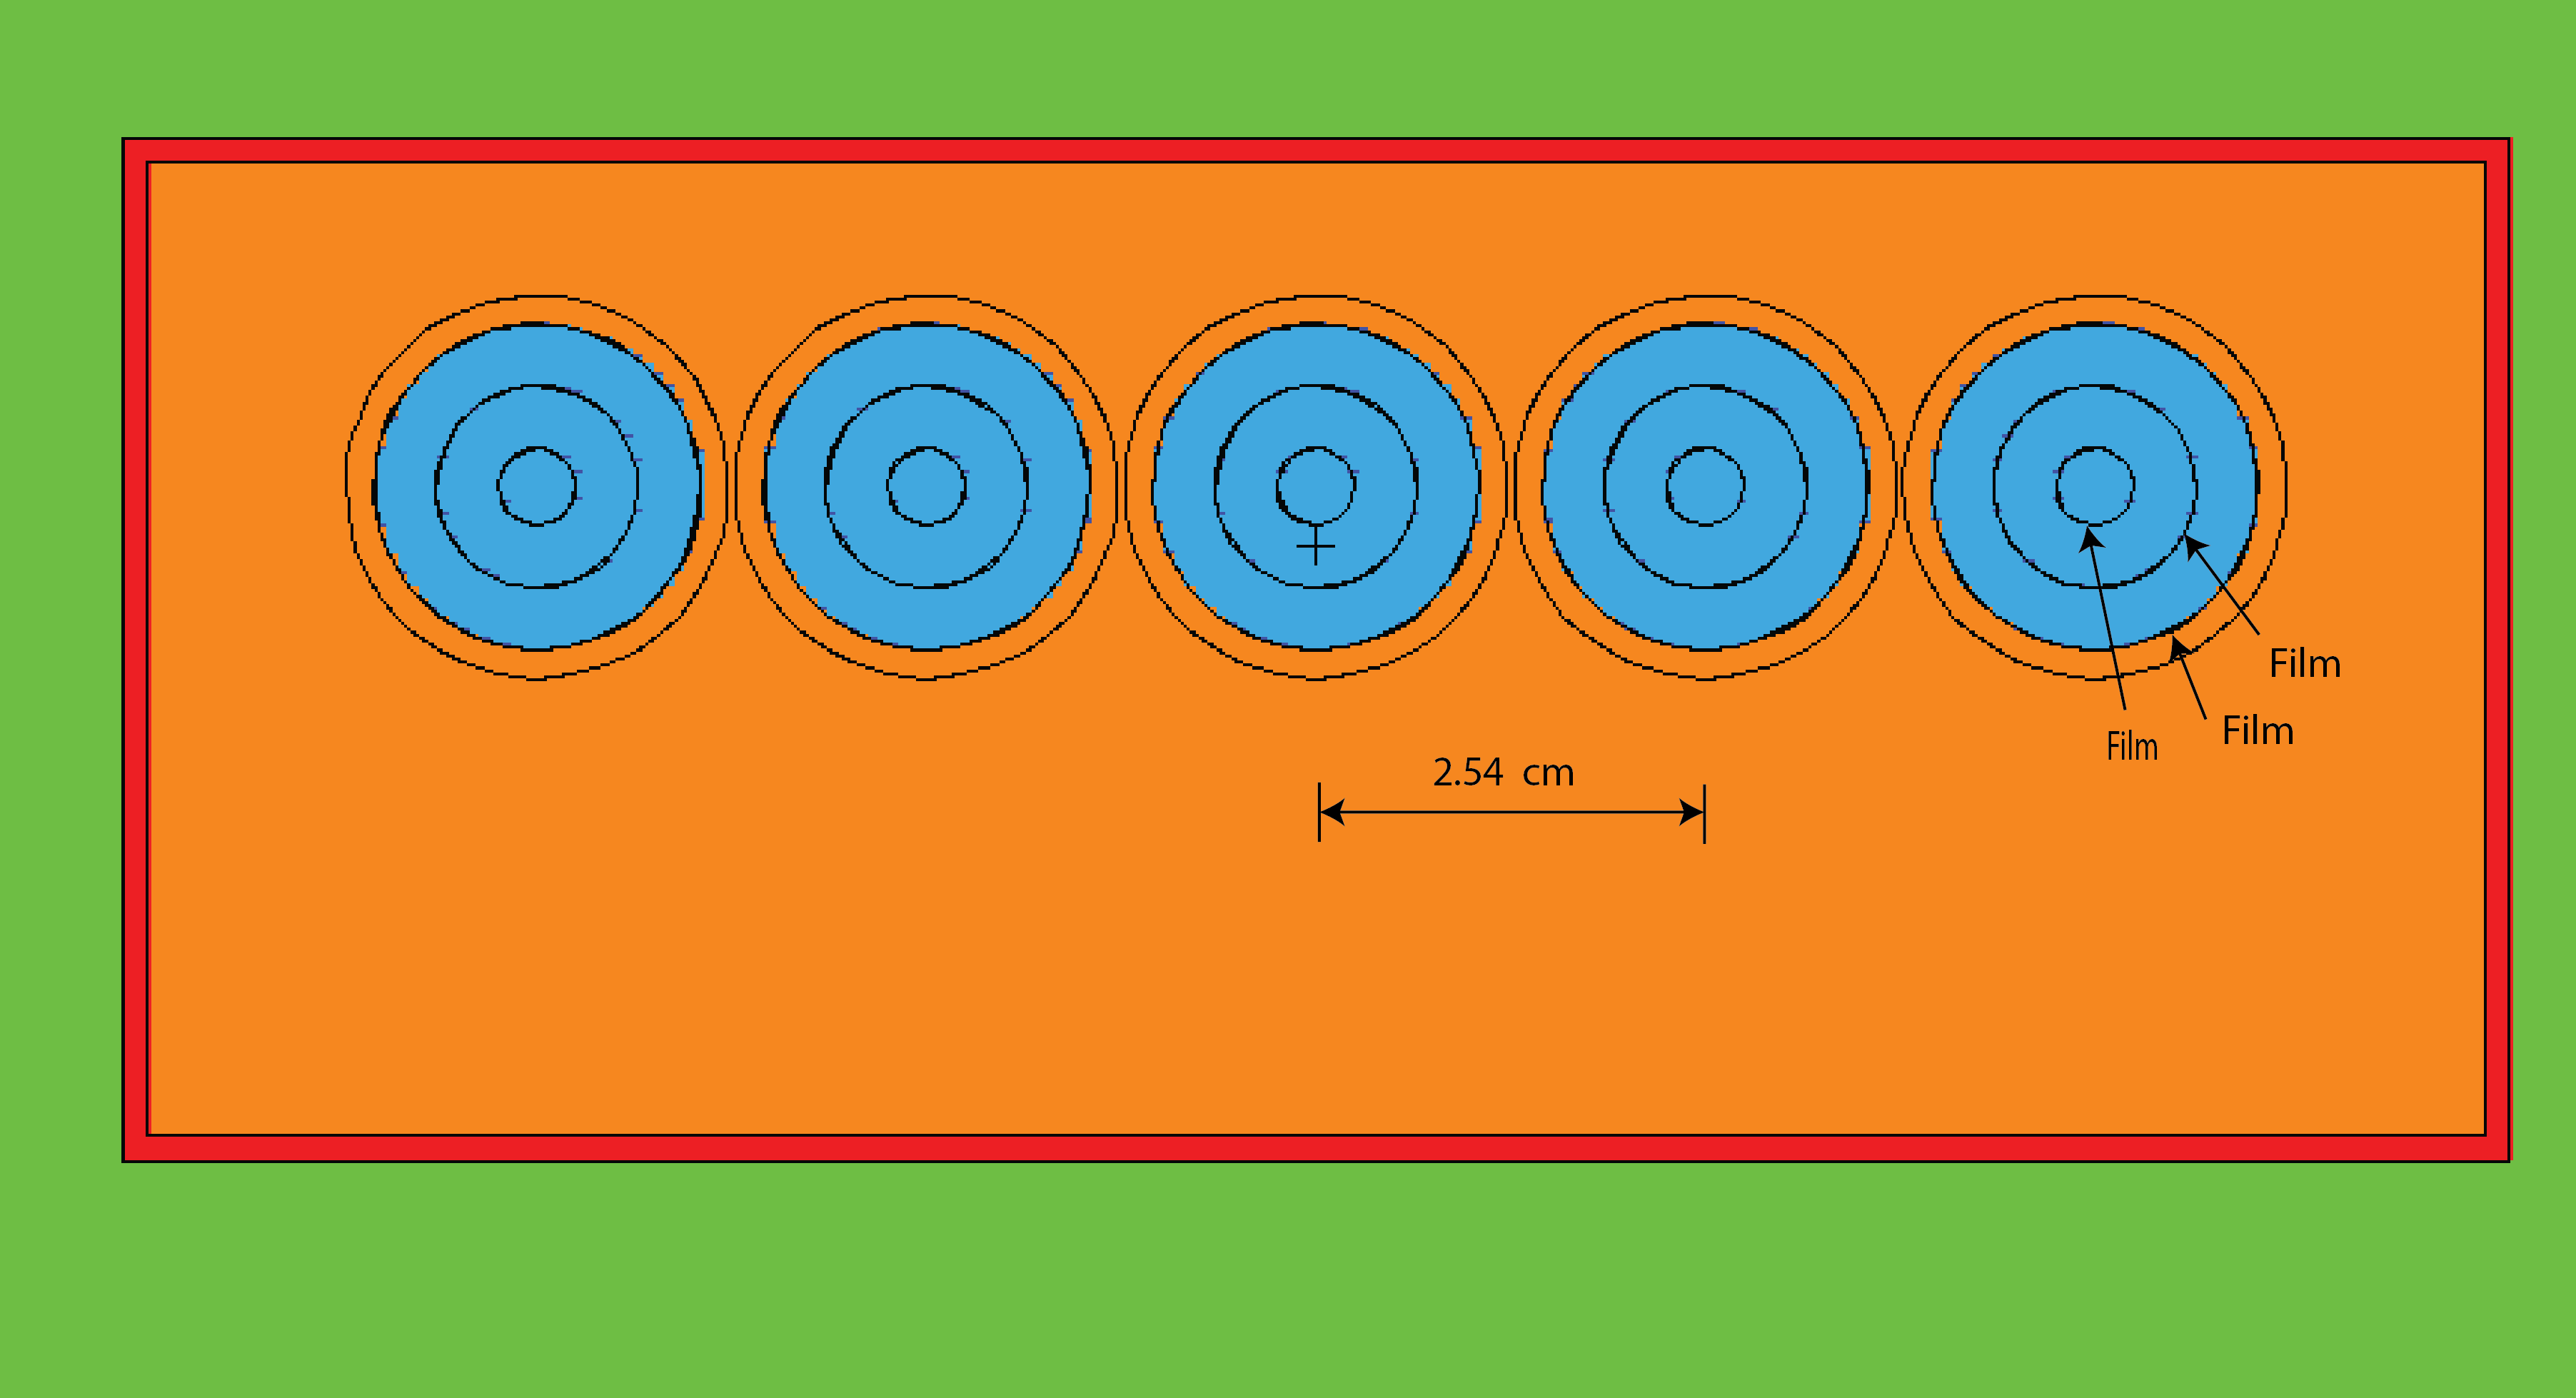
\includegraphics[width=\textwidth,height=\textheight,keepaspectratio]{WrappedGeoCylinder_FiveCylinders}
  \caption[Rendering of Five Layered Cylinders in RPM Cabinet]{MCNPX Rendering of five wrapped cylinders placed in an RPM8 Cabinet. The spacing between the detector layers is \SI{0.8}{\cm}, with the total detector having an interaction rate of  \SI{2.92}{cps\per\ng  \iso[255]{Cf}}.}
  \label{fig:FiveLayerCylinderGeo}
\end{figure}

The five cylinder design (with \SI{0.8}{\cm} spacing between detector film layers) had three layers of detectors in each of the five cylinders.
The inner most layer, with an inner radius of \SI{0.5}{\cm}, contained 13\% of the mass \iso[6]{Li}, while the second layer contained 33\%  and the outer layer (inner radius \SI{2.12}{\cm}) contained the majority of the absorber at 54\%.
The interaction rate of each detector film layer in a cylinder is described for all five cylinders in \autoref{tab:WrappedCylinderRXNRate}.
It is observed that the outer cylinder (located at $\pm$ \SI{10.16}{\cm})reaction rates are very similar to the other three, suggesting that the edges effect and the flux depression due to presences of the other cylinders are negligible.
In addition, it is observed that when the interaction rate is normalized by the fraction that each cylinder occupies in the assembly there is little difference (beyond the 5\% statistical convergence on the tallies) in the reaction rate per unit mass between the layers, thus suggesting a close to optimal material usage is achieved.
If it was necessary, however, to trim material the inner cylinder would be an ideal candidate due to contributing little in the way of total counts.
In this design the outer cylinders had over 56\% of the total interaction rate, while the innermost cylindrical film layers contributed less than 12\% to the total interaction rate.
\begin{table}
	\caption[Neutron Interactions per Layer in Cylinder]{Simulated Interaction rate (per nanogram \iso[252]{Cf}). The tally convergence was within 5\% for all tally values.}
	\label{tab:WrappedCylinderRXNRate}
	\begin{tabular}{m{4cm} | m{2cm} m{1.75cm} m{1.5cm} m{1.5cm} m{1.5cm}}
		\toprule
		Fraction of Assembly & \SI{-10.16}{\cm} & \SI{-5.08}{\cm} & \SI{0}{\cm} & \SI{5.08}{\cm} & \SI{10.16}{\cm}\\
		\midrule
		0.13 & 0.072 & 0.074 & 0.069 & 0.070 & 0.062 \\
		0.33	& 0.180 & 0.201 & 0.186 & 0.189 & 0.172 \\
		0.54	& 0.318 & 0.351 & 0.330 & 0.338 & 0.310 \\
		\bottomrule
	\end{tabular}
\end{table}
